
\documentclass[dvips,12pt,openright,a4paper,final]{report}

%\documentclass[leftflush,openright,a4paper,12pt,fleqn]{report}
\usepackage{supertabular}
\usepackage{fancyhdr}
\usepackage[english]{babel}
\usepackage{amssymb}
\usepackage{amsmath}
\usepackage{subfigure}
\usepackage[dvips]{graphicx,color}
\usepackage{makeidx}
\usepackage{nomencl}
\usepackage{cite}
\usepackage{graphicx}
\usepackage{amsmath,amsfonts}
\usepackage{longtable}
\usepackage{afterpage}
\usepackage{graphicx}
\usepackage{datetime}
\usepackage{lipsum}
\usepackage{enumitem}
\usepackage[left=2cm,right=2cm,top=2cm,bottom=2cm]{geometry}
\usepackage{ragged2e}
\usepackage{amsmath}
\usepackage{float}
\restylefloat{table}
%\floatstyle{boxed} 
\restylefloat{figure}



%%%%%%%%%%%%%%%%%%%%%%%%%%%%%%%%%%%%%%%%%%%%
\thispagestyle{empty}
\input intmacros.sty
%%%%%%%%%%%%%%%%%%%%%%%%%%%%%%%%%%%%%%%%%%%%
\renewcommand{\baselinestretch}{1.2}
\setlength{\textheight}{9.2in}
\setlength{\textwidth}{6.1in}
\addtolength{\leftmargin}{-.3in}
\topmargin -.2in
\pagenumbering{}
%%%%%%%%%%%%%%%%%%%%%%%%%%%%%%%%%%%%%%%%%%%%
\usepackage{pslatex}
\begin{document}
\pagestyle{empty}

\begin{center}
\renewcommand{\baselinestretch}{2}


\vspace{.4in}
{\large \bf A PROJECT REPORT ON}\\
 \vspace { 5mm}
 
{\large \bf "HIERARCHICAL OPTIMIZATION OF OPTIMAL PATH\\
 FINDING IN TRANSPORTATION APPLICATIONS"} \\
\textbf{Under The Guidance of}\\
\textbf{Prof. U.R.GODASE}\\
\vspace{.2in}
\textbf{BY}\\
\vspace{.2in}
\begin{tabular}{rl}
\textbf{ASHWINI MORE}\textbf{(B8238586)} & \textbf{PUNAM NERKAR}\textbf{(B8238589)}\\
\textbf{RAMOLA NIKAM}\textbf{(B8238591)}  & \textbf{SHRADHA PIDHEKAR}\textbf{(B8238605)  } \\
\end{tabular}\\
\vspace{.3in}
IN THE PARTIAL FULFILLMENT OF THE REQUIREMENTS 
FOR THE AWARD OF THE DEGREE\\[1mm]
OF\\[1mm]
\textbf{BACHELOR OF ENGINEERING\\ 
(INFORMATION TECHONOLOGY)}
\vspace{.1in}


{\large \bf AT}\\
\vspace{.3in}
\centering
		
\vspace{.1in}
\begin{figure}[htp]
\hspace*{5 cm}

\includegraphics[scale=1]{STES.png}
\end{figure}

{\bf DEPARTMENT OF INFORMATION TECHONOLGY}\\
\vspace{.1in}
{\bf SINHGAD COLLEGE OF ENGINEERING,PUNE 411041}\\
\hspace*{3 cm}\textbf{Affilated to}
\vspace{.1in}
\begin{figure}[htp]
\hspace*{6 cm}

\includegraphics[scale=1]{inpune.jpg}
\end{figure}
\newline
\textbf{UNIVERSITY OF PUNE}
\end{center}
   

\newpage
\pagestyle{plain}
\pagenumbering{roman}

\newpage
\input{CERTIFICATE}


\newpage
\addcontentsline{toc}{chapter}{ABSTRACT}
\begin{center}
{\Large \bf Abstract}
\end{center}
\vspace{5mm}

%\begin{flushright}
%\begin{flushleft}
\justifying
%\lipsum[1]
\hspace{1cm}
	Efficient path query processing is a key requirement for advanced database applications including GIS (Geographic Information Systems) and ITS (Intelligent Transportation Systems). We study the problem in the context of automobile navigation systems where a large number of path requests can be submitted over the transportation network within a short period of time. To guarantee efficient response for path queries, we employ a path view materialization strategy for precomputing the best paths. We tackle the following three issues: (1) memory-resident solutions quickly exceed current computer storage capacity for networks of thousands of nodes, (2) disk based solutions have been found inefficient to meet the stringent performance requirements, and (3) path views become too costly to update for large graphs. Proposed HEPV(Hierarchical Encoded Path View) approach addresses these problems while guaranteeing the optimality of path retrieval.

%\end{flushleft}
%\end{flushright}

\newpage
\addcontentsline{toc}{chapter}{ACKNOWLEDGEMENT}
\begin{center}
{\LARGE \bf Acknowledgement}
\end{center}
\vspace{5mm}

%\begin{flushleft}
\justifying
%\lipsum[1]
\hspace{1cm}
	It is our privilege to acknowledge with deep sense of gratitude towards all, who gave us the possibility of completing this project. We would also like to express our sincere gratitude to our project guide,Prof.U.R.Godase for her valuable suggestions and guidance throughout our course of study and timely help given for completing project.\\
\hspace*{1cm}This project would not have been possible without the support of our H.O.D. Prof. A. W. Rohankar and our principal Prof. S.D.Lokhande. Their knowledge and assistance has always been supportive and helpful throughout the course of our Bachelor of Engineering.\\
\hspace*{1cm}Special thanks to our colleagues for providing the support in developing the project, who backed our interest by giving useful and timely suggestions and for sharing the literature and invaluable assistance.\\
\hspace*{1cm}We wish to express love and gratitude to our families; for their understanding and moral support.\\

%\end{flushleft}
\vspace{5mm}
\begin{flushright}

Date: \ddmmyyyydate \today
%Date:19/10/2011   \\
\end{flushright}
\begin{flushright}       
Place:\hspace*{1cm} Pune \\
\end{flushright}

\listoffigures
\tableofcontents


%\listoftables
%\listofabbreviations
%%\newpage
%%\input{symbols}
%%\newpage
%%\input{abbreviations}

%%%%%%%%%%%%%%%
%\pagestyle{plain}
%\pagestyle{headings}
%\pagenumbering{arabic}
%
\pagestyle{fancy}
\pagenumbering{arabic}
% it will occur at top i.e. header
\lhead{} % this is for left header
\chead{} % this is for center header
\rhead{} % this is for right header
%it will occur at bottom i.e. footer
\lfoot{} % this is for left footer
\cfoot{\tiny SCOE,Information Technology\\(2011-12).}% this is for center footer
\rfoot{\thepage} % this is for right footer
\renewcommand{\headrulewidth}{0.0pt} % draw & set line possition for header
\renewcommand{\footrulewidth}{0.4pt} % draw & set line possition for footer
\newpage % insert new page
\newpage
\pagestyle{fancy}
\pagenumbering{arabic}

%\begin{flushleft}

\justifying
\chapter{\large INTRODUCTION}


\section{\normalsize BACKGROUND}


\hspace{1cm}In early days,it was much difficult for an individual to travel from one place to another.To reach a particular destination,while travelling at every turn he had to ask other person for the right path.This was quite time consuming and a reason for unnecessary extra fare at times if he go in a wrong way.\\
\hspace*{1cm}So to overcome these  problems and to reach the particular destination in lesser time with optimal path,this idea emerged.By using this HEPV algorithm,we can get the most optimum path between any two places.\\
\subsection{Basic Concepts}
\textbf{a) FlatGraph :}
\\
\hspace*{1cm}The graph of nodes and links where nodes represents the places
and links represents the path is called the flat graph.
\\
\textbf{b) Local Node :}
\\
\hspace*{1cm}The node which is present in only one fragment is called as 
	local node.
\\
\textbf{c) Border Node :}
\\
\hspace*{1cm}The node which is present in more than one fragment is called as border node.\\
\textbf{d) Fragments :}
\\
\hspace*{1cm}The flat graph is divided into smaller graphs to create a  
hierarchy of a graph are called as fragments.
\\
\hspace*{1cm}In our project we are taking flat graph of 30 nodes. The nodes are as follows:
\\

\hspace{0.5cm}1.	Pune  Station
\\ \hspace*{1cm}2.	Sanchetee  Hospital
\\ \hspace*{1cm}3.	Shivaji  Nagar
\\ \hspace*{1cm}4.	Manapa
\\ \hspace*{1cm}5.	Shaniwar Wada
\\ \hspace*{1cm}6.	Swargate
\\ \hspace*{1cm}7.	Hirabaug  Bus stop
\\ \hspace*{1cm}8.	Bharti  Vidyapith
\\ \hspace*{1cm}9.	Saras  Baug
\\ \hspace*{1cm}10.	Katraj
\\ \hspace*{1cm}11.	Balgandharv
\\ \hspace*{1cm}12.	Crompton Greaves
\\ \hspace*{1cm}13.	Aundh
\\ \hspace*{1cm}14.	FC
\\ \hspace*{1cm}15.	Garware  Chowk
\\ \hspace*{1cm}16.	Dandekar  Pool
\\ \hspace*{1cm}17.	Nal  Stop
\\ \hspace*{1cm}18.	Mhatre  Pool
\\ \hspace*{1cm}19.	Karnataka School
\\ \hspace*{1cm}20.	Tathawade  Udyan
\\ \hspace*{1cm}21.	Rajaram Pool
\\ \hspace*{1cm}22.	Tukai  Nagar
\\ \hspace*{1cm}23.	Kothrud  Depo
\\ \hspace*{1cm}24.	Karve  Putala
\\ \hspace*{1cm}25.	Kothrud Stand
\\ \hspace*{1cm}26.	Karve Nagar
\\ \hspace*{1cm}27.	Meenakshi Puram
\\ \hspace*{1cm}28.	SCOE
\\ \hspace*{1cm}29.	Vadgaon BK
\\ \hspace*{1cm}30.	Aanand  Nagar
\\
\newpage
\hspace*{1cm}The flat graph looks like as given in next figure�
\\
\begin{figure}[H]
\vspace*{-1.2in}
	\centering
		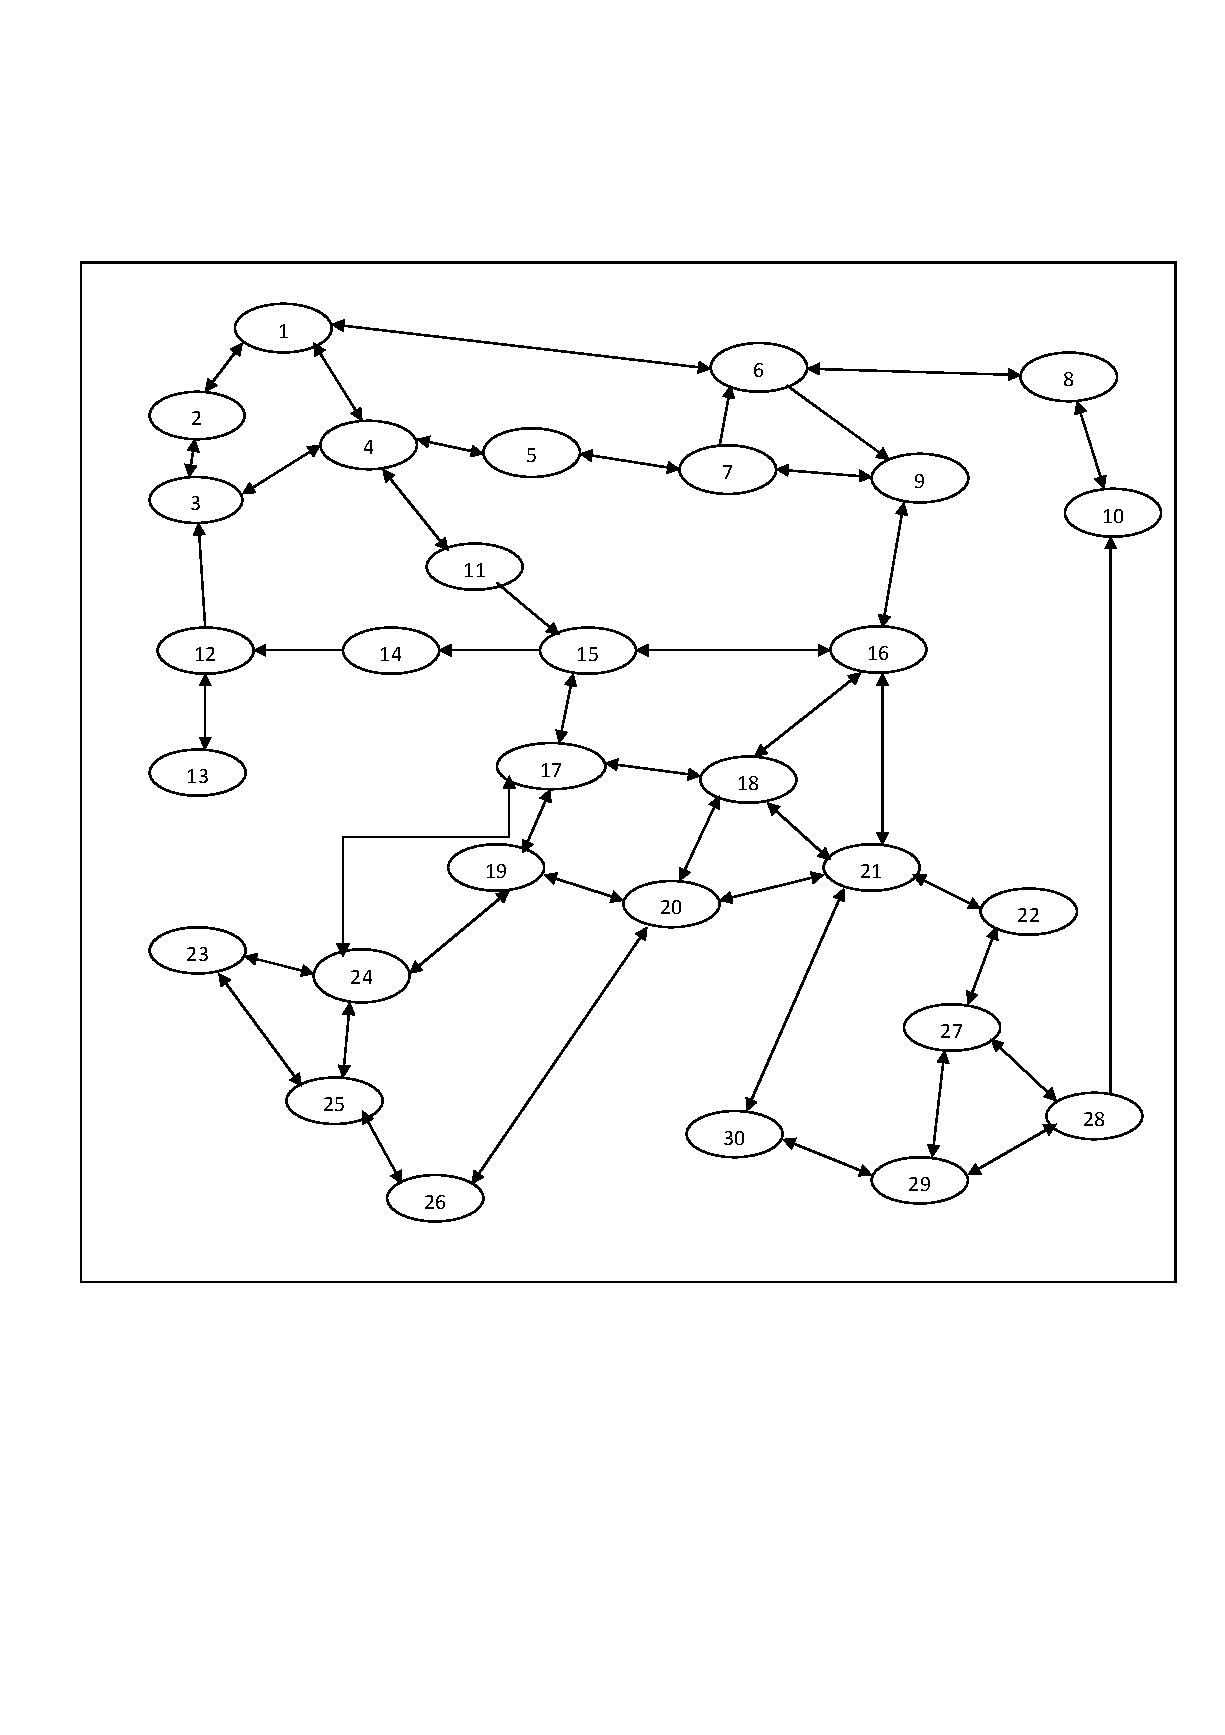
\includegraphics[width=13cm,height=16cm]{flat.eps}
	\vspace{-1.5in}	\caption{Flatgraph}
	\label{fig:flat}
\end{figure}

\hspace*{1cm}Above figure shows the graphical representation of selected area. It is called as flat graph. The flat graph is divided into partitions. In our project we have only 1 partition and 4 fragments of that partition. The figures of fragments are as shown below.\\

\newpage
\begin{figure}[H]
\vspace{-1.2in}
	\centering
		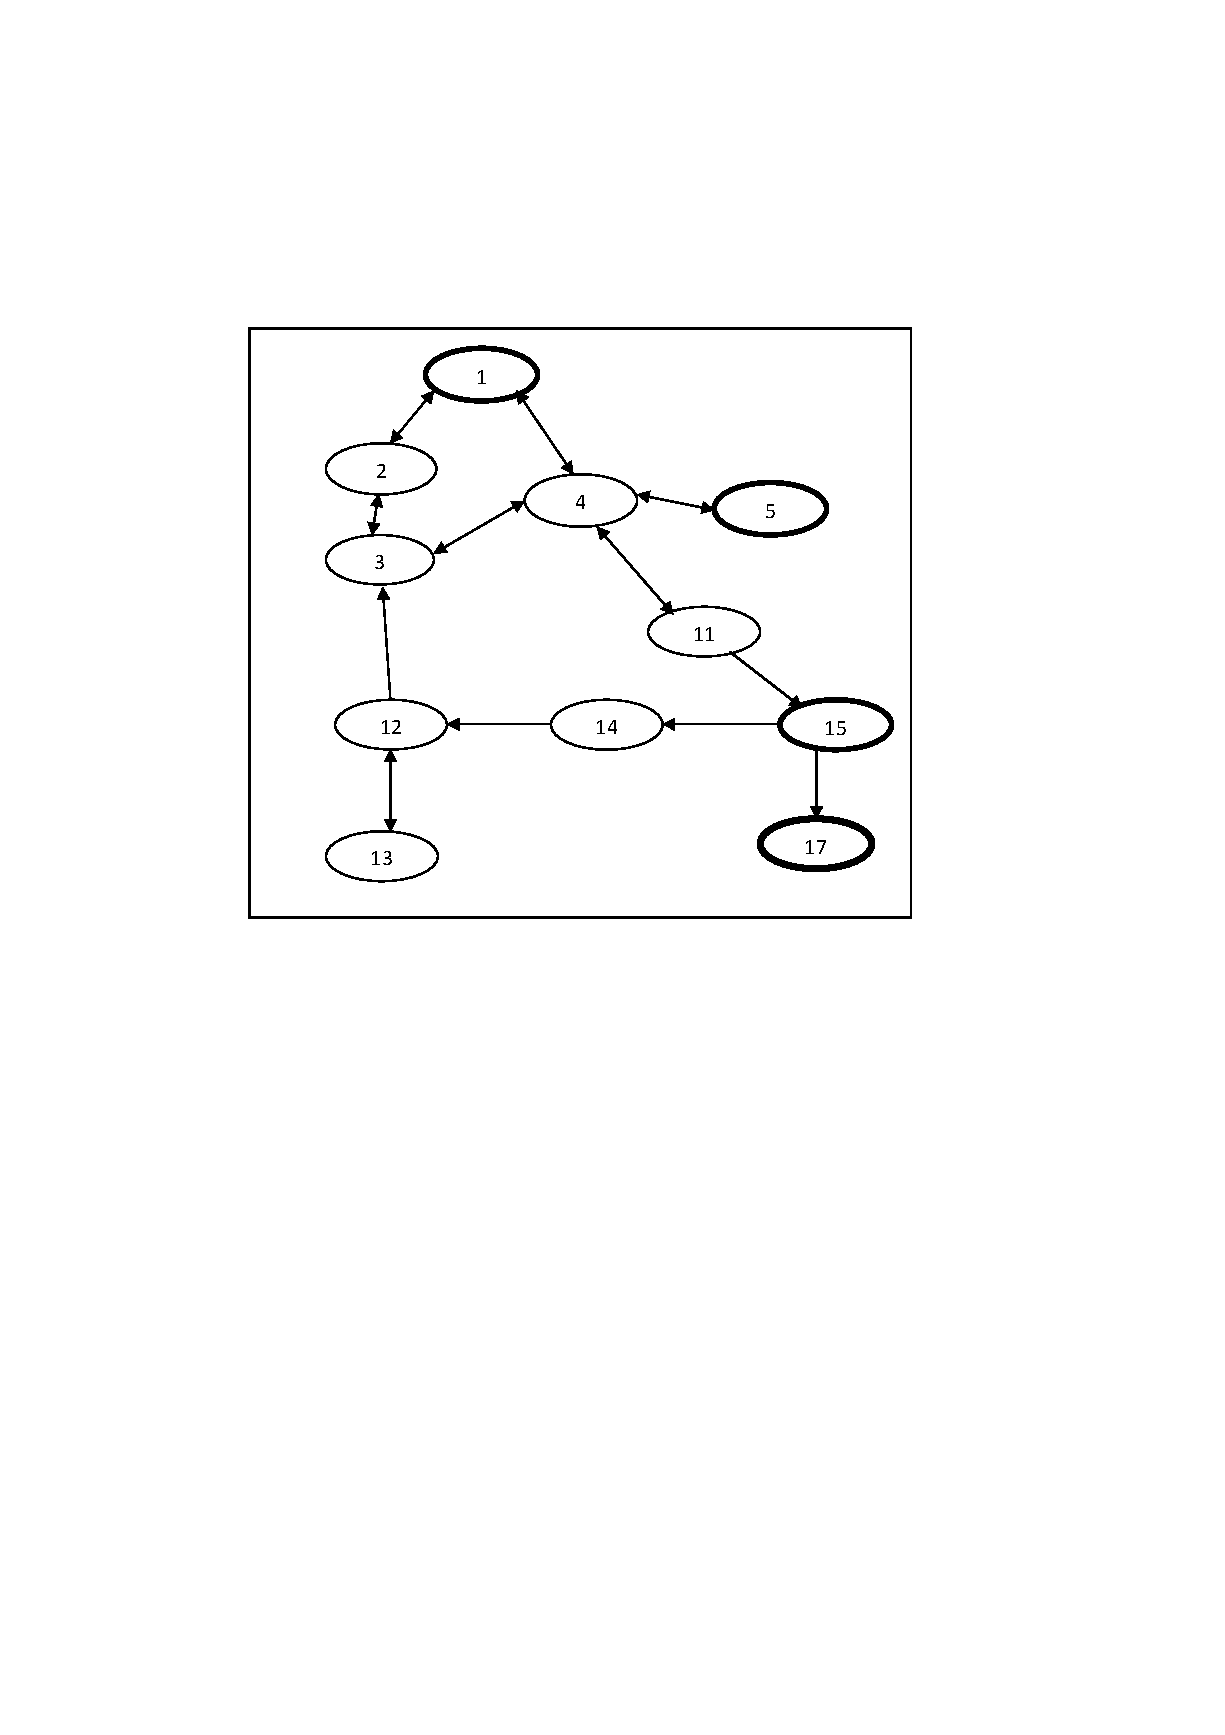
\includegraphics[width=10cm,height=13cm]{frag1.eps}
	\vspace{-1.5in}	\caption{Fragment1}
	\label{fig:frag1}
\end{figure}

\begin{figure}[H]
\vspace{-1.1in}
	\centering
		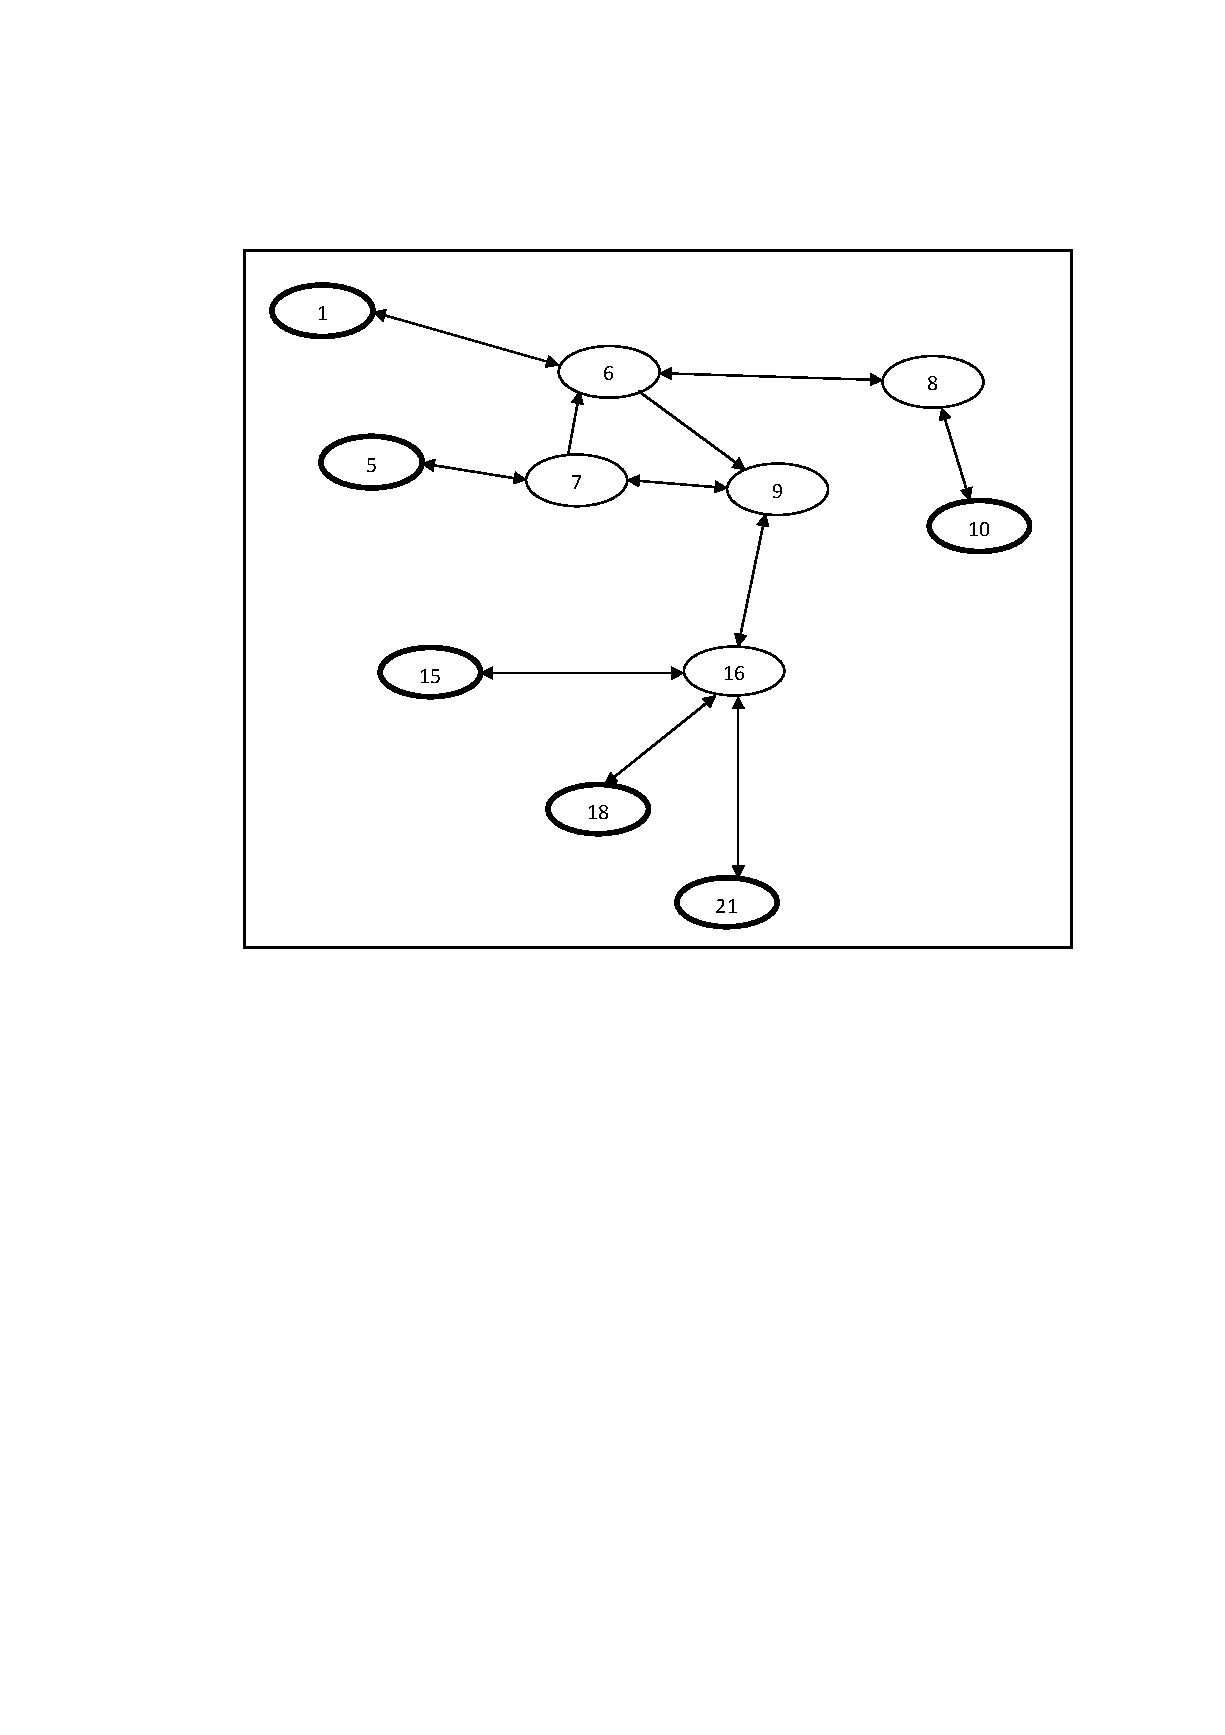
\includegraphics[width=10cm,height=13cm]{frag2.eps}
	\vspace{-1.5in}	\caption{Fragment2}
	\label{fig:frag2}
\end{figure}
\newpage

\begin{figure}[H]
\vspace{-1.4in}
	\centering
		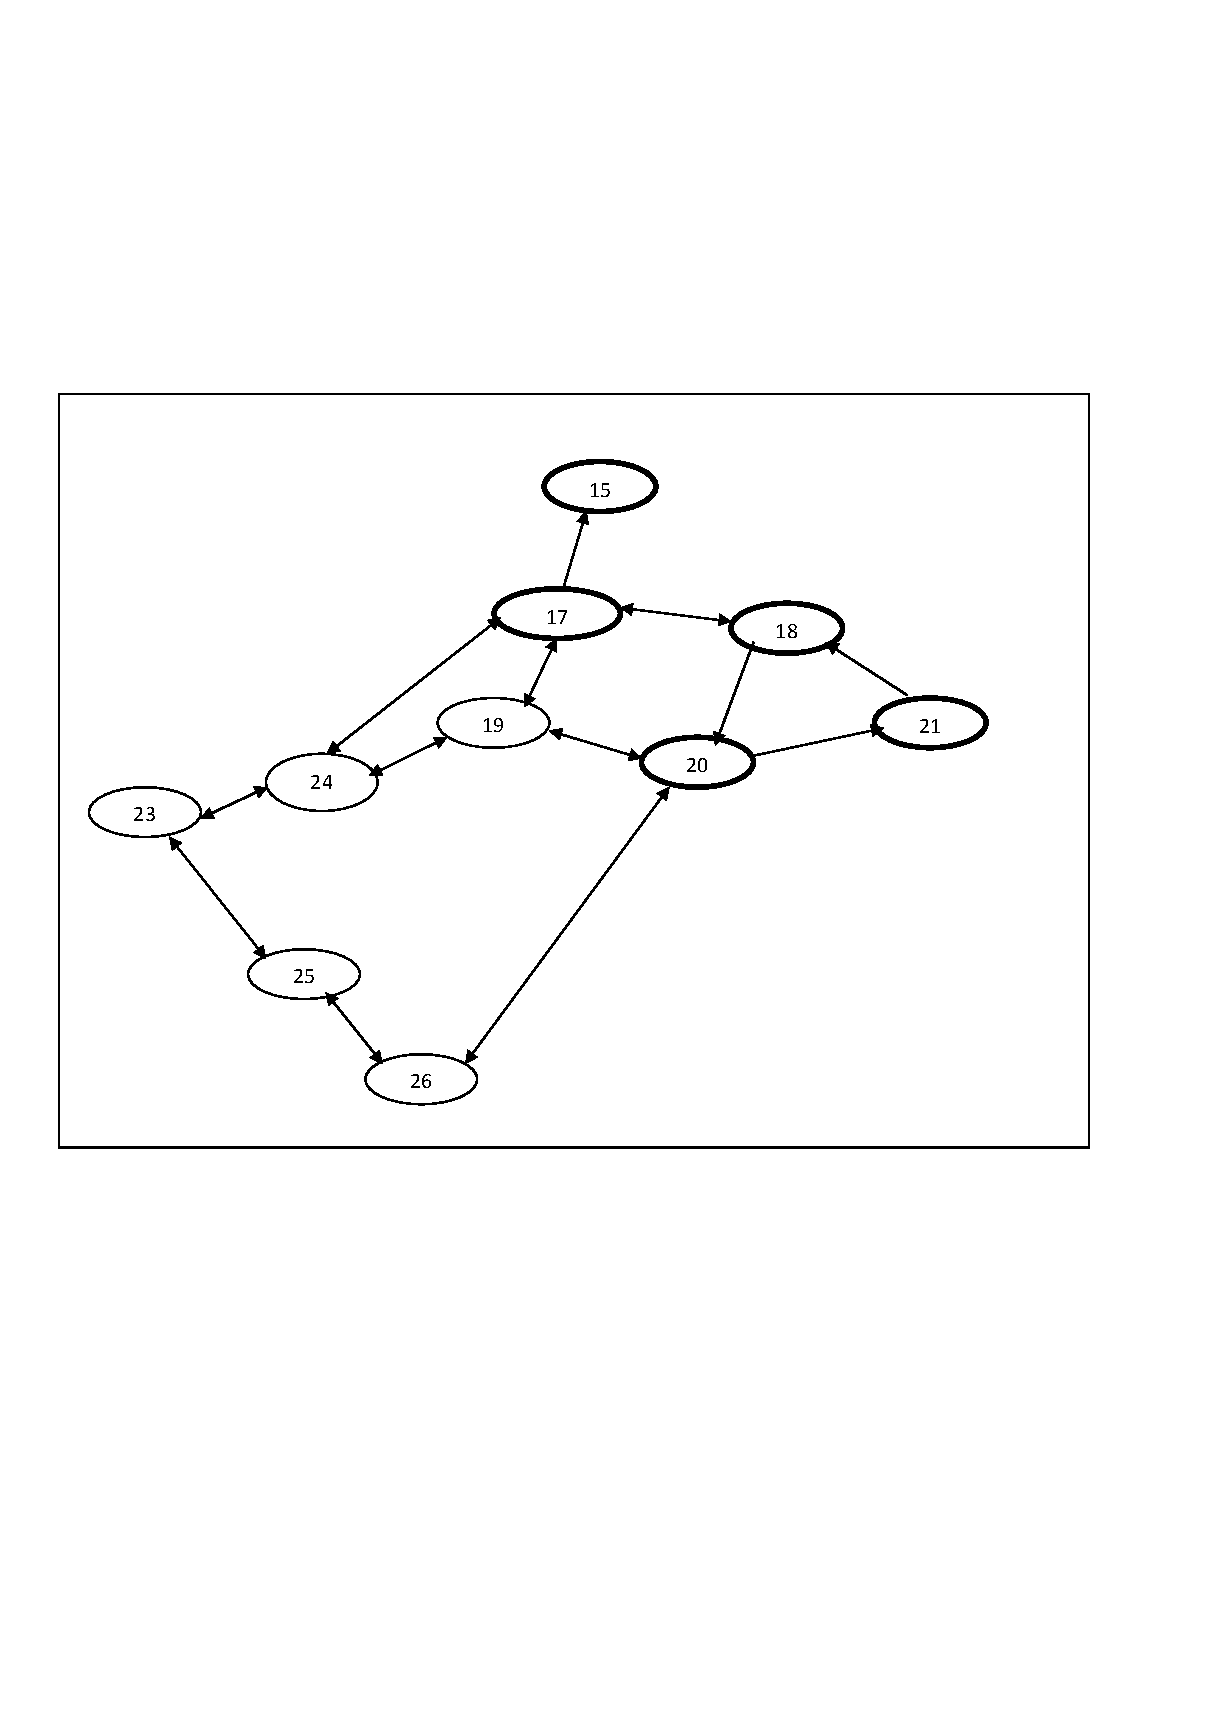
\includegraphics[width=10cm,height=13cm]{frag3.eps}
	\vspace{-1.5in}	\caption{Fragment3}
	\label{fig:frag3}
\end{figure}

\begin{figure}[H]
\vspace{-1.2in}	
	\centering
		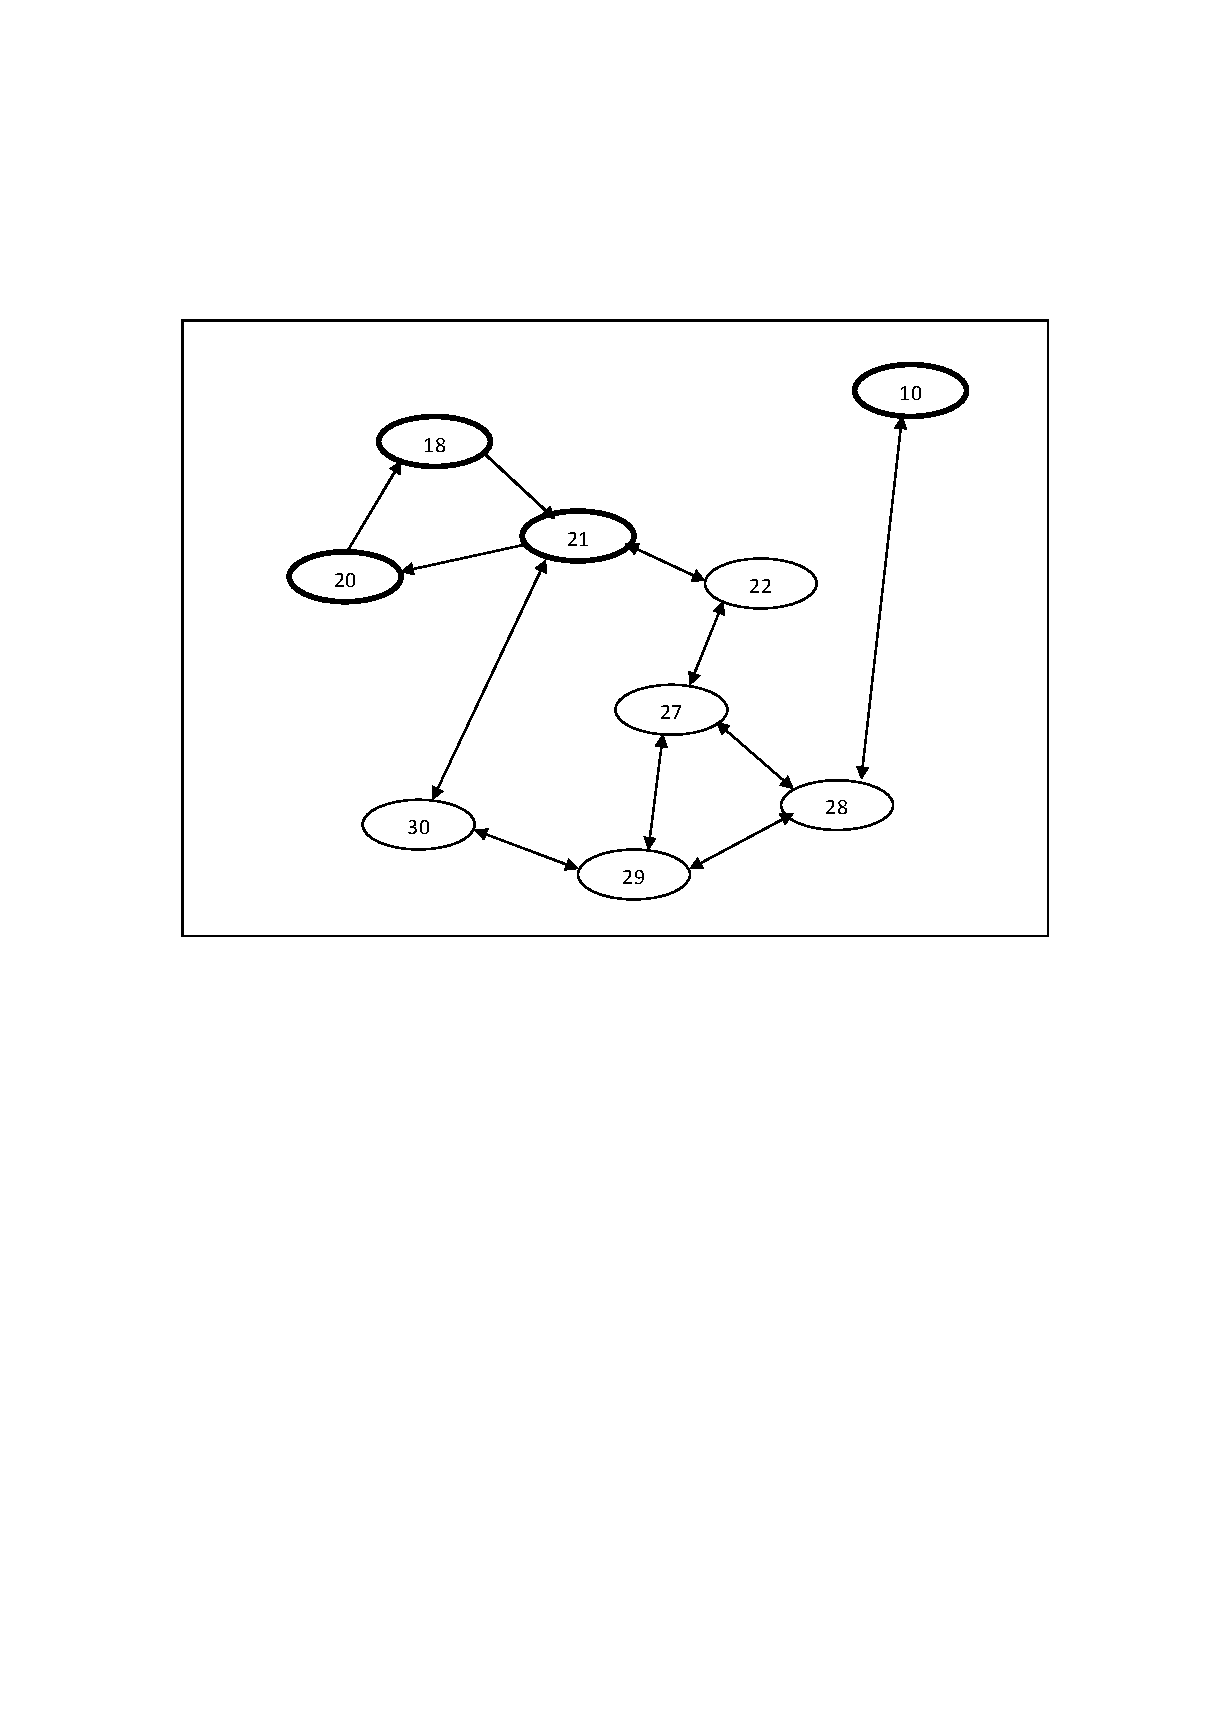
\includegraphics[width=10cm,height=13cm]{frag4.eps}
	\vspace{-1.5in}	\caption{Fragment4}
	\label{fig:frag4}
\end{figure}

\hspace*{1cm}The nodes which are highlighted are border nodes and remaining are local nodes. First we divide the flat graph into no. of small graphs and then by taking a border nodes we create a super graph, which is used to find the optimal path between source and destination. Thus we create a hierarchy of graph. \\

\newpage
\section{\normalsize LITERATURE SURVEY}
%\justifying

\hspace{1cm}Dijikstra algorithm is used to compute the shortest path between two nodes. It calculates the path on demand. It does not precompute the path.  It does not use the concept of fragments. It does not guarantee the optimal solution. It can not handle the large graphs. Thus it is not efficient algorithm for shortest path finding.
\\
\hspace*{1cm}Transitive closure algorithm[2,3] precomputes the paths between source and destination. It does not use fragment also it does not guarantee optimality of a solution.  Theoretically it can handle the huge graph but while much research has been conducted by both the theory and database communities on path finding, many suggested transitive closure algorithms do not effectively handle path computation on large graphs in real-time application domains such as ITS (Intelligent Transportation Systems) systems. With new computer architectures and networks, the traditional algorithms were adapted to parallel and distributed transitive closure algorithms[5].\\
\hspace*{1cm}As an alternative approach, precompute all-pair shortest paths and store them in an encoded path view structure. Queries can be efficiently answered by performing simple lookups on the precomputed path view. This approach is a trade-off between computing paths from scratch and precomputing all paths. While this approach has been proven to be promising for relatively small map data sets, it was determined that it exceeds the memory capacity of typical computer systems for large graphs (e.g., graphs of 3,600 nodes or larger) and the performance of computing the path view deteriorates quickly (e.g., it takes 4 minutes for a graph with 3,600 nodes on a Sun SPARC-20).\\
\hspace*{1cm}The hierarchical abstraction has been proposed by some researchers to overcome this problem[5]. for example divided a relation into fragments and introduced the notion of high-speed fragment. Unfortunately, the formation of high speed fragments are very sensitive to the update of the underlying base relation. Therefore the authors recommended this approach only for rather stable base relations. Some researches have presented a hierarchical graph model which classifies links according to road types and pushes up high speed roads such as highways to the next higher level of hierarchy. However, the paths retrieved from such hierarchical graphs are not guaranteed to be optimal.\\
\hspace*{1cm}A hierarchical A* algorithm for road navigation systems, which while more efficient than flat A* does not guarantee optimality either. It can handle large graph. It uses both the techniques of precomputation and on demand computation.\\
\hspace*{1cm} Similarly, some other researchers proposed another hierarchical multigraph model by dividing graph into subgraphs and pushing up the precomputed paths as well as links between the boundary nodes. The paper did not discuss how the optimality can be achieved. Hierarchical graph refreshing essential for road navigation to reflect the dynamic traffic condition was also not handled.\\


\section{\normalsize PROBLEM DEFINITION}
\subsection{Software Requirement Specification}
\textbf{Problem Statement:}\\
%\justifying
\hspace*{1cm}To find an optimal path for an individual to travel in an alien place such that intermediate nodes are revealed. The capability of computing path queries is an essential feature for advanced database applications. Our goal is to explore solutions for path finding in general with particular focus on addressing the problems inherent to navigation systems applications.
\vspace{.2in}\\
\textbf{Intended Audience and Reading Suggestions:}\\
%\justifying
\hspace*{1cm}This SRS is used by developers, project managers, marketing staff, users, testers and documentation writers for different purposes like developer refers this SRS for coding, testers to build test plans, marketing staff for deciding marketing strategies. This SRS also contains scope of the project, references, project features etc.
\vspace{.2in}\\
\textbf{Project Scope:}\\
%\justifying
\hspace*{1cm}This system is developed under windows environment in JAVA�.. Simple database are used and also simple program files are used. There are separate files for each transaction. 
\\
\hspace*{1cm}1.	We are concerned with providing answers to path queries issued by a potentially large number of concurrent requests (e.g., during peak rush hour periods).
\\ \hspace*{1cm}2.	Our solution must handle the dynamic nature of transportation networks, i.e., it must provide up-to-date query results even when the underlying transportation networks change frequently.  
\\ \hspace*{1cm}3.	Our solution must provide response at a near real-time level of performance (i.e., within seconds). 
\\ \hspace*{1cm}4.  Based on the requirements of instruction based navigation systems, we are interested in efficiently determining the next link for the desired path rather than necessarily retrieving the complete path all at once.
\vspace{.2in}\\
\textbf{Product Perspective:}\\
%\justifying
\hspace*{1cm}The product is standalone application and It is neither a distributed nor a client-server system. 
\vspace{.2in}\\
\textbf{Product Features:}\\
%\justifying
\hspace*{1cm}
1.	Optimal Path
\\
\hspace*{1cm}2.	Intermediate nodes
\vspace{.2in}\\
\textbf{User Classes and Characteristics:}\\
%\justifying
\hspace*{1cm}1.	User-requires some knowledge about computers. How to use the system.
\\	
\hspace*{1cm}2.	Employee should be well trained to handle the application. He/she must know all the features and functions of this software,so he can update the database.
\vspace{.2in}\\
\textbf{Operating Environment :}\\
%\justifying
\hspace*{1cm}Windows operating system 
\vspace{.2in}\\
\textbf{Design and Implementation Constraints:}\\
\hspace*{1cm}Databases to be used : Oracle 10g\\
\hspace*{1cm}Language requirements : JAVA
\vspace{.2in}\\
\textbf{User Documentation:}\\
%\justifying
\hspace*{1cm}User manuals, help ,CD and tutorials
\vspace{.2in}\\
\textbf{Assumptions and Dependencies:}\\
%\justifying
\hspace*{1cm}The graph of interconnected places within city is predefined .This graph can be modified depending on requirement. The computer system on which our product is installed should have sufficient resources to store this information.\\
\hspace*{1cm}We assume that our product does not provide networking capabilities. It is a standalone application.

\vspace{.15cm}
\newpage
\subsection{Project Plan}


%\end{flushleft}
%\begin{center}
 %   \begin{tabular}{| l | p{8cm} | l | l | l |}
 %   \hline
 %  \textbf{ No.}  &	\textbf{Task} &	\textbf{Starting} &	\textbf{Finish} & \textbf{No.of days}\\ %\hline
%   1 &	Project selection &	16/07/2011 &	11/08/2011 & 26 \\ \hline
%   2 & Discuss about various projects &	16/07/2011 & 23/07/2011 & 7 \\ \hline
%   3 &	Project topic searching &	23/07/2011 &	02/08/2011 &	10\\ \hline
%4 &	“Hierarchical Optimization of Optimal Path Finding for
%Transportation Applications” as a project. & 03/08/2011 & 03/08/2011 &	1\\ \hline
%5 & Synopsis creation &  04/08/2011	& 11/08/2011 &	8\\ \hline
%6 & 1st Review &	24/08/2011	& 24/08/2011 &	1\\ \hline
%7 & Approval of project	& 24/08/2011 &	24/08/2011 &	1\\ \hline
%8 & Information gathering &	25/08/2011	& 19/09/2011 &	25\\ \hline
%9	& Collecting required  documents &	25/08/2011	&      2/09/2011 &	8\\ \hline
%10 &	Study of IEEE papers and references &	30/08/2011 &	17/09/2011 &	18\\ \hline
%11	& Estimate resources required	& 12/09/2011 &	19/09/2011	& 8\\ \hline
%12	 & Documentation and designing &	17/09/2011	& 4/10/2011 &	17\\ \hline
%13 &	UML ,DFD , Activity Diagrams &	17/09/2011	& 4/10/2011	& 17\\ \hline
%14	& 2nd  Review & 	05/10/2011	 & 05/10/2011 &	1\\ \hline
%15 &	SRS generation &	05/10/2011 &	06/10/2011 &	2\\ \hline
%16	& Partial Report generation &	05/10/2011	& 07/10/2011 &	3\\ \hline
%    \end{tabular}
%\end{center}


\newpage
%\begin{flushleft}


\chapter{\large PROJECT PLANNING AND MANAGEMENT}

\section{\normalsize PROJECT DEVELOPMENT LIFECYCLE}
\justifying
\begin{center}
\begin{figure}[hbtp]
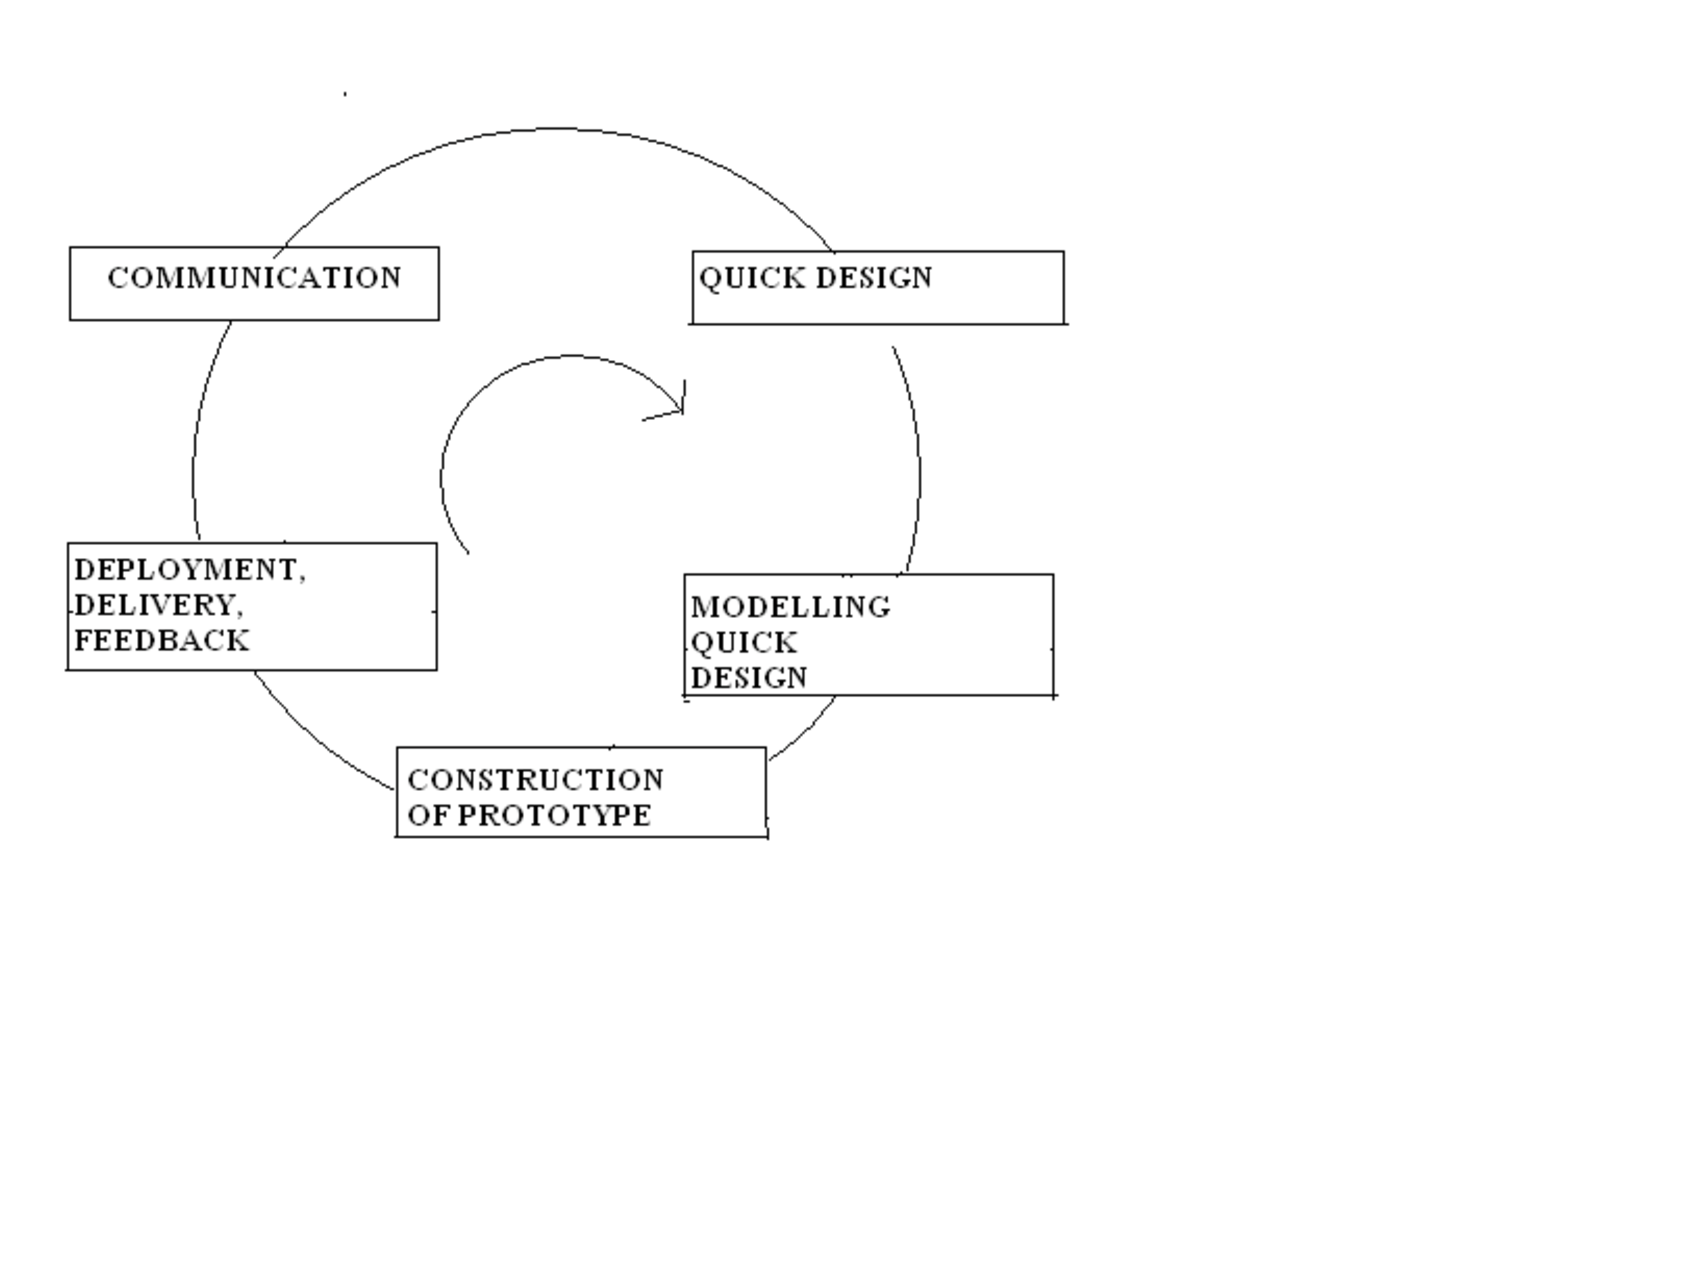
\includegraphics[width=20cm,height=13cm]{pdl.eps}
\caption{Project Devlopment Life Cycle}
\end{figure}
\end{center}
\newpage
\textbf{1. Requirement Gathering:}\\
\hspace*{1cm}The project development lifecycle starts with understanding all the requirements of the system. It involves the communication between the user and the developer. Based upon the functionalities of the system and the points stated by the end user the requirements of the project are decided. It also involves generating the Software Requirement Specification (SRS).\\
Requirement of project is – \\
\hspace*{1cm}1.	Flatgraph with numbered nodes, weight\\
\hspace*{1cm}2.	Database that stores the flatgraph, partition and supergraph\\
\hspace*{1cm}3.	GUI that makes path viewing easier\\
\hspace*{1cm}4.	Authentication of user for security\\
\hspace*{1cm}5.	Platform Independent language to be used for coding
\vspace{.2in}\\
\textbf{2.Planning:}\\
\hspace{1cm}The planning phase includes complete estimation and scheduling of the activities to be performed in the project. It includes the distribution of work, the estimated time to complete the project, the estimated cost, job scheduling and tracking.\\
\hspace{1cm}
Information gathering, study of IEEE papers and estimation of resources required is completed before beginning of documentation and designing.\\
\hspace{1cm}
After completion of documentation and design project work will be evenly distributed in team. Team will first study the project flow. Database being less complex will be designed precisely by one team member. Then another team member will work on the gui design. The other two members will begin with coding part. All these sections have to start simultaneously.\\
\hspace{1cm}
Project will be divided roughly into 3 phases. Phase 1 has to be completed till mid December. Phase 2 has to be completed till January end and Phase 3 has to be completed till February end.
\vspace{.2in}\\
\textbf{3.Modeling and Design:}\\
\hspace*{1cm}It includes detail requirement analysis and project design. It also involves development of  algorithms and various architectural concepts like use case diagrams, flowcharts  etc.\\
\hspace*{1cm}
Use Case Diagram, Class Diagram, DFD, ERD, Activity Diagram, Sequence Diagram and State Transition Diagram are designed before 2nd Review. Complete detailing and flow of project is demonstrated by these diagrams.\\

\textbf{Project is divided in 3 phases –}\\
\hspace*{1cm}\textbf{Phase 1-}\\
\hspace*{1cm}
Algorithms will be thoroughly studied before beginning of database design. Flatgraph will be designed and module will be designed to encode the flatgraph. The encoded flatgraph will be stored in database.\\
\hspace*{1cm}
Gui will be developed. Authentication for system security will be designed.\\
\hspace*{1cm}\textbf{Phase 2-}\\
\hspace*{1cm}
After encoding the flatgraph into database coding for partition and supergraph must begin. Database design for storing partition and supergraph will be done. \\
\hspace*{1cm}
Gui for creating, encoding partition and supergraph will be designed simultaneously.\\
\hspace*{1cm}\textbf{Phase 3-}\\
\hspace*{1cm}
During coding of path retrieval normalization of database and perfection of gui will be carried out.
Development of Path Retrieval module will be time consuming thus in this phase focus will be mainly on path retrieval module.
\vspace{.2in}\\
\textbf{4.Construction:}\\
It includes coding and testing steps:\\
\hspace*{1cm}
1.	Coding: Design details are implemented using appropriate programming language.\\
\hspace*{1cm}
2.	Testing: Testing is carried out to check whether flow of coding is correct and to point out the errors of the program.\\
Coding will be done in following steps –\\
\hspace*{1cm}
1.	Encoding flatgraph\\
\hspace*{1cm}
2.	Authentication of user\\
\hspace*{1cm}
3.	Create and encode partition\\
\hspace*{1cm}
4.	Develop gui for the same\\
\hspace*{1cm}
5.	Create and encode supergraph\\
\hspace*{1cm}
6.	Develop gui for the same\\
\hspace*{1cm}
7.	Develop path retrieval module\\
\hspace*{1cm}
8.	Develop gui for usage of customer\\

Testing will be done with overall gui and algorithms. Testing will be performed timely and before deployment of project.
\vspace{.2in}\\
\textbf{5.Deployment:}\\
	\hspace*{1cm}It includes software delivery , support and feedback from user. If the user suggests some corrections, or demands additional capabilities then changes are required for such corrections or enhancements.  \\
\hspace*{1cm}
	Deployment will be done after complete testing of the project.\\


\section{\normalsize PROJECT DELIVERABLES}


Deliverables for our project will include:\\
1.\textbf{Project report}\\
\hspace*{1cm}It includes Software Requirement Specification, All design details, technical diagrams, schedule, cost, testing details etc..\\
2.\textbf{CD}\\
\hspace*{1cm}It contains the Hierarchical Optimization Of Optimal Path Finding System GUI set up.\\
3.\textbf{Manual}\\
\hspace*{1cm}Provides all procedures required while using the system. Also contains the Help.
\\

\section{\normalsize TASKS AND MILESTONES}
\subsection{Tasks}
\textbf{The following tasks have to be performed:}\\
\hspace*{1cm}1.	Database with tables required for flat-graph, partitions and supergraph will be created.\\
\hspace*{1cm}2.	Authentication mechanism will be developed.\\
\hspace*{1.5cm}Admin only is allowed to create, encode partitions and supergraph.\\
\hspace*{1cm}3.	Modules to create and encode partitions and supergraph will be developed.\\
\hspace*{1cm}4.	Optimal Path Retrieving module will be developed.\\

\subsection{Milestones}
	\hspace*{1cm}In general the following major milestones can be considered "completed"� when the criteria noted have been met.\\
	
1)  Development of different modules:
   It is necessary to divide the project in different modules and work on those modules individually.
 
2)	Testing of modules individually:
 The modules which are developed are then tested one at a time. All the elements related to a module are tested and if needed modification is done at that time.
 
 3)	 Module Integration :
    After all the modules are tested individually they are combined to form the whole project.

4)	Testing Project as a Whole :
    After integrating the modules the project is tested as a whole to see if any bugs are left. They are rectified then and the project is then ready for Deployment.


5)	Follow up of Guidelines :
    It is seen that all Guidelines given are maintained and all the expectations of the user from the application are fulfilled. Also the application should be user friendly.

\vspace{.2in}
\textbf{Hierarchical Optimization of Optimal Path Finding System will have following}\\
\vspace*{0cm}\textbf{milestones:}\\
\hspace*{1cm}1.	Authentication of Admin\\
\hspace*{1cm}2.	Creation and encoding of Partitions from flatgraph\\
\hspace*{1cm}3.	Creation and encoding of Supergraph from partitions\\
\hspace*{1cm}4.	Maintenance of Hierarchical Encoded Path View(HEPV)\\
\hspace*{1cm}5.	Optimal Path Retrival using Hierarchical Encoded Path View(HEPV)\\

\section{\normalsize COST AND EFFORT ESTIMATION}
\hspace{1cm}The constructive Cost Model is generally used for estimation measure of project cost, project duration, manpower etc.\\
\hspace*{1cm}Like all estimation models, the COCOMO model requires sizing information .This information can be specified in terms of:
\begin{description}
\item[\hspace*{1cm}$\bullet$]Object Point(OP)
\item[\hspace*{1cm}$\bullet$]Function Point(FP)
 \item[ \hspace*{1cm}$\bullet$]Lines Of Source Code(KLOC)
  \end{description}
For our project we use sizing information in the form of line of source code(KLOC).
\begin{description}
\item[\hspace*{1cm}$\bullet$]Total lines of code for our Project,KLOC = 3.6k(approx)
\item[\hspace*{1cm}$\bullet$]Cost of each person per month Cp = Rs.1500/-(approx)
\end{description}

\textbf{Efforts} \\
\hspace*{1cm}Equation for calculation of efforts in person-months for COCOMO model is:\\
\hspace*{3.5cm} E = a*(KLOC)$^{b}$\\
\hspace*{1cm}Where,\\
 \hspace*{1.5cm}a=3.0\\
  \hspace*{1.5cm}b=1.12\\
   \hspace*{1.5cm}E=Efforts in person-months\\
\hspace*{3.5cm}E=3.0*(3.6)$^{1.12}$\\
\hspace*{3.5cm}E=12.59 person-months\\
\hspace*{1cm}Total efforts of 12.59 person-months are required to complete the project successfully\\

\textbf{Duration of Project:}\\ 
\hspace*{1cm}Equation for calculation of Duration of projects in months for COCOMO model is:\\
\hspace*{3.5cm} D = A * (E)$^{b}$ \\
 \hspace*{1cm}Where,\\
\hspace*{1.5cm}a=2.5\\
\hspace*{1.5cm}b=0.32\\
\hspace*{1.5cm}D=Duration of Project in months.\\
\hspace*{3.5cm}D=2.5*(12.59)$^{0.32}$ \\

\hspace*{1cm}The approximate duration of project is 5.63 months\\

\textbf{Number of team members:}\\
 \hspace*{1cm}The equation for calculation of Number of team members required for completion of project, using COCOMO model is:\\
\hspace*{3.5cm}N = E / D\\

\hspace*{1cm}Where,\\
 \hspace*{1.5cm}N=number of team members required.\\
 \hspace*{1.5cm}E=Efforts in person-months.\\
  \hspace*{1.5cm}D=Duration of project in months.\\
 \hspace*{3.5cm}N=12.59/5.63\\
 \hspace*{3.5cm}N=3  (approx)\\

\textbf{Cost of project:}\\
 \hspace*{1cm}Equation for calculation of cost of project, using COCOMO model is:\\
\hspace*{3.5cm} C = D * Cp\\
	
\hspace*{1cm} Where,\\
\hspace*{1.5cm}	C=Cost of Project.\\
 \hspace*{1.5cm} D=Duration of Project in Months.\\
 \hspace*{1.5cm}Cp=Cost incurred per person-month\\
\hspace*{3.5cm}C=5.63 * 6400\\

\hspace*{1.5cm}Therefore total cost of project is Rs. 36032 /-(approx)\\

		 

\section{\normalsize RISKS}
\subsection{Technical Risks:}
\hspace*{1cm}No technical risks as such is existing since the Operating System being used is Windows, which is well established as well as accepted. Maintenance problem could exist in system.
\subsection{Product Size Risks:}
\hspace*{1cm}The size estimate in LOC of our project may be significantly low. This may affect the schedule as well as upset the estimate and total cost of our project. 

\subsection{Business Risks:}
\hspace{1cm}The top five business risks are \\
\hspace*{1cm}1)	Building an excellent product or system that nobody really wants (market risk).\\
\hspace*{1cm}2)	Building a product that no longer fits into the overall business strategy for the company (strategy risk).
\\ \hspace*{1cm}3)	Building a project that the sales force does not understand how to sell.
\\ \hspace*{1cm}4)	Losing the support of senior management due to a change in focus or change in people (management risk).
\\ \hspace*{1cm}5)	Losing budgetary or personnel commitment (budget risk).

\subsection{System Failure}
\hspace*{1cm}If Database crash during the path retrieval then it is tedius task to recover the database. 

%\end{flushleft}
%\begin{flushleft}
\begin{center}

\chapter{\large PROJECT ANALYSIS}

\justifying
\section{\normalsize USE CASE MODEL WITH SCENARIOS}
\vspace*{2mm}
\hspace{5mm} A Use case diagram captures use case and actor interactions.There are two level of use case diagram one context  level and other is requirement level.\\

\justifying
\subsection{\small Use Case level 0}
\vspace*{2mm}
\hspace{5mm}Here is the use case model level 0\\
\begin{figure}[H]
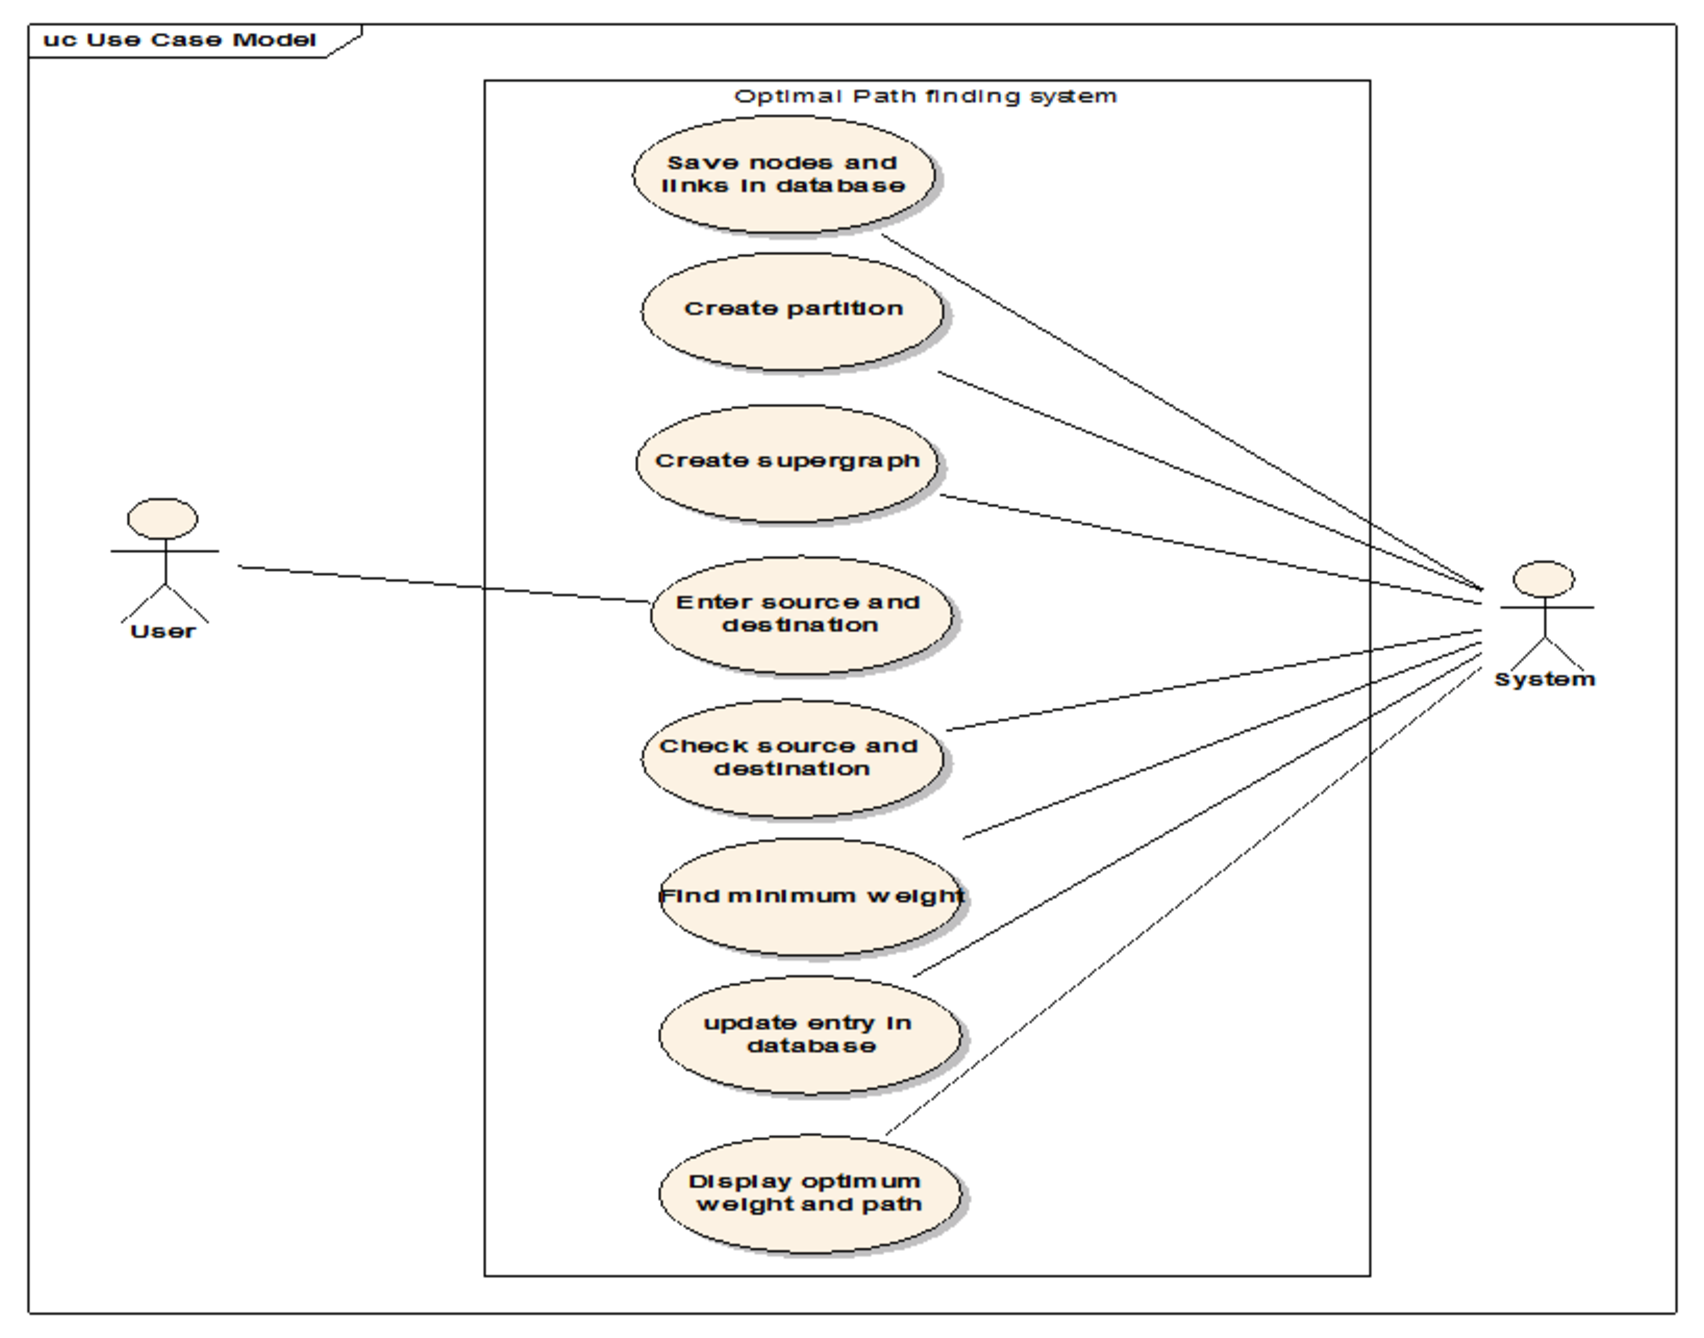
\includegraphics[width=13cm,height=8cm]{usecase0.eps}
\caption{Use Case Level 0}
\end{figure}
%\newpage


\subsection{\small Use Case level 1}
\begin{figure}[H]
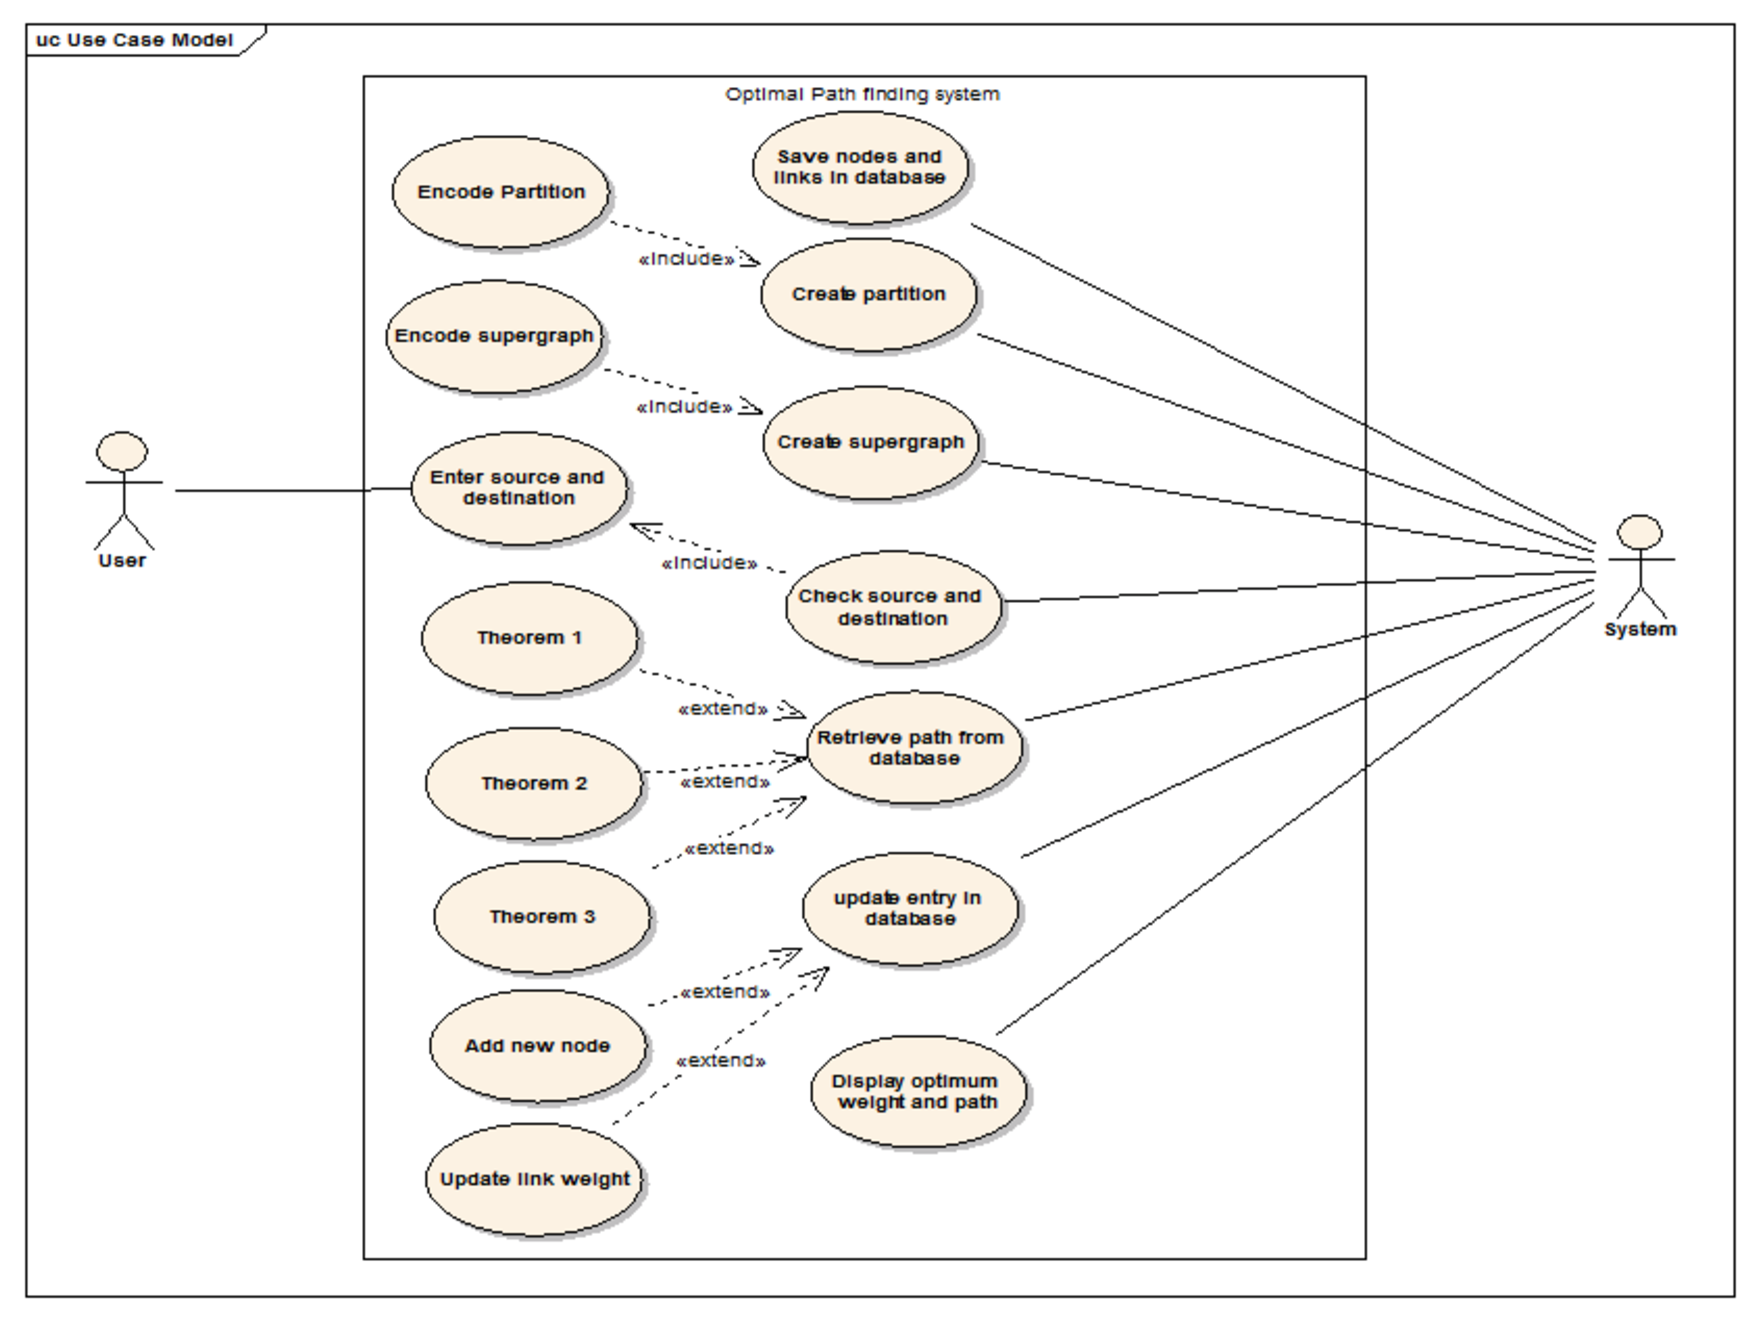
\includegraphics[width=15cm,height=16cm]{usecase1.eps}
\caption{Use Case level 1}
\end{figure}
\newpage

\section{\normalsize ACTIVITY DIAGRAM}
\hspace*{5mm}Activity diagrams are used to model the behaviours of a system, and the way in which these behaviours are related in an overall flow of the system. The logical paths a process follows, based on various conditions, concurrent processing, data access, interruptions and other logical path distinctions, are all used to construct a process, system or procedure.\\

\begin{figure}[H]
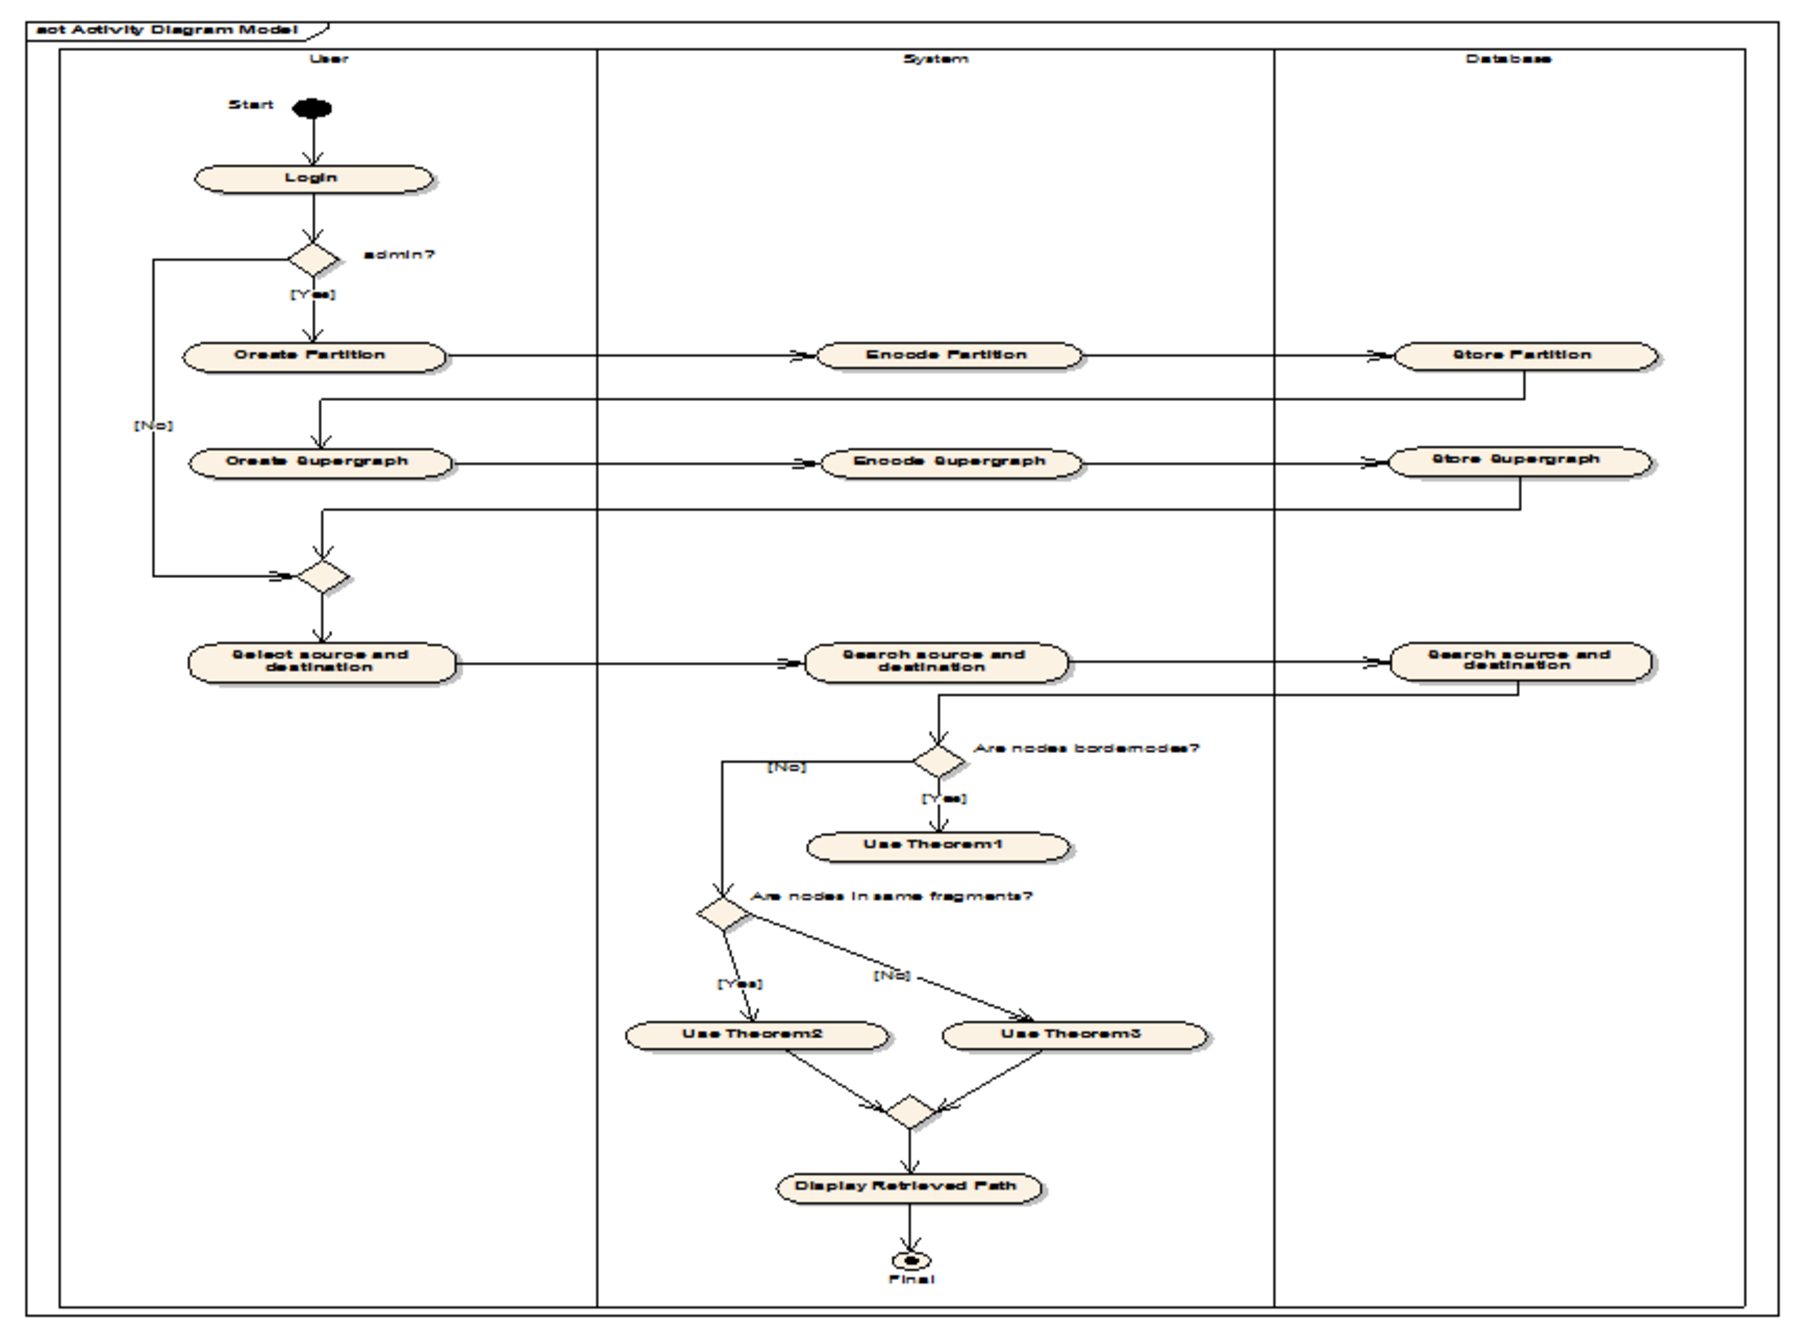
\includegraphics[width=16cm,height=13cm]{act.eps}
\caption{Activity Diagram}
\end{figure}
%\newpage
\end{center}
%\end{flushleft}


\begin{center}

\justifying
\chapter{\large PROJECT DESIGN}

\justifying
\section{\normalsize DATAFLOW DIAGRAM LEVEL 0}
\hspace{5mm} A data flow diagram (DFD) is a graphical representation of the "flow" of data through an information system, modeling its process aspects. Often they are a preliminary step used to create an overview of the system which can later be elaborated. DFDs can also be used for the visualization of data processing (structured design.\\
\hspace{5mm} DFD shows interaction between external entities and processes and process and data store.\\
%\\ \hspace*{1cm} Following is the Dataflow diagram level 0
\begin{figure}[H]
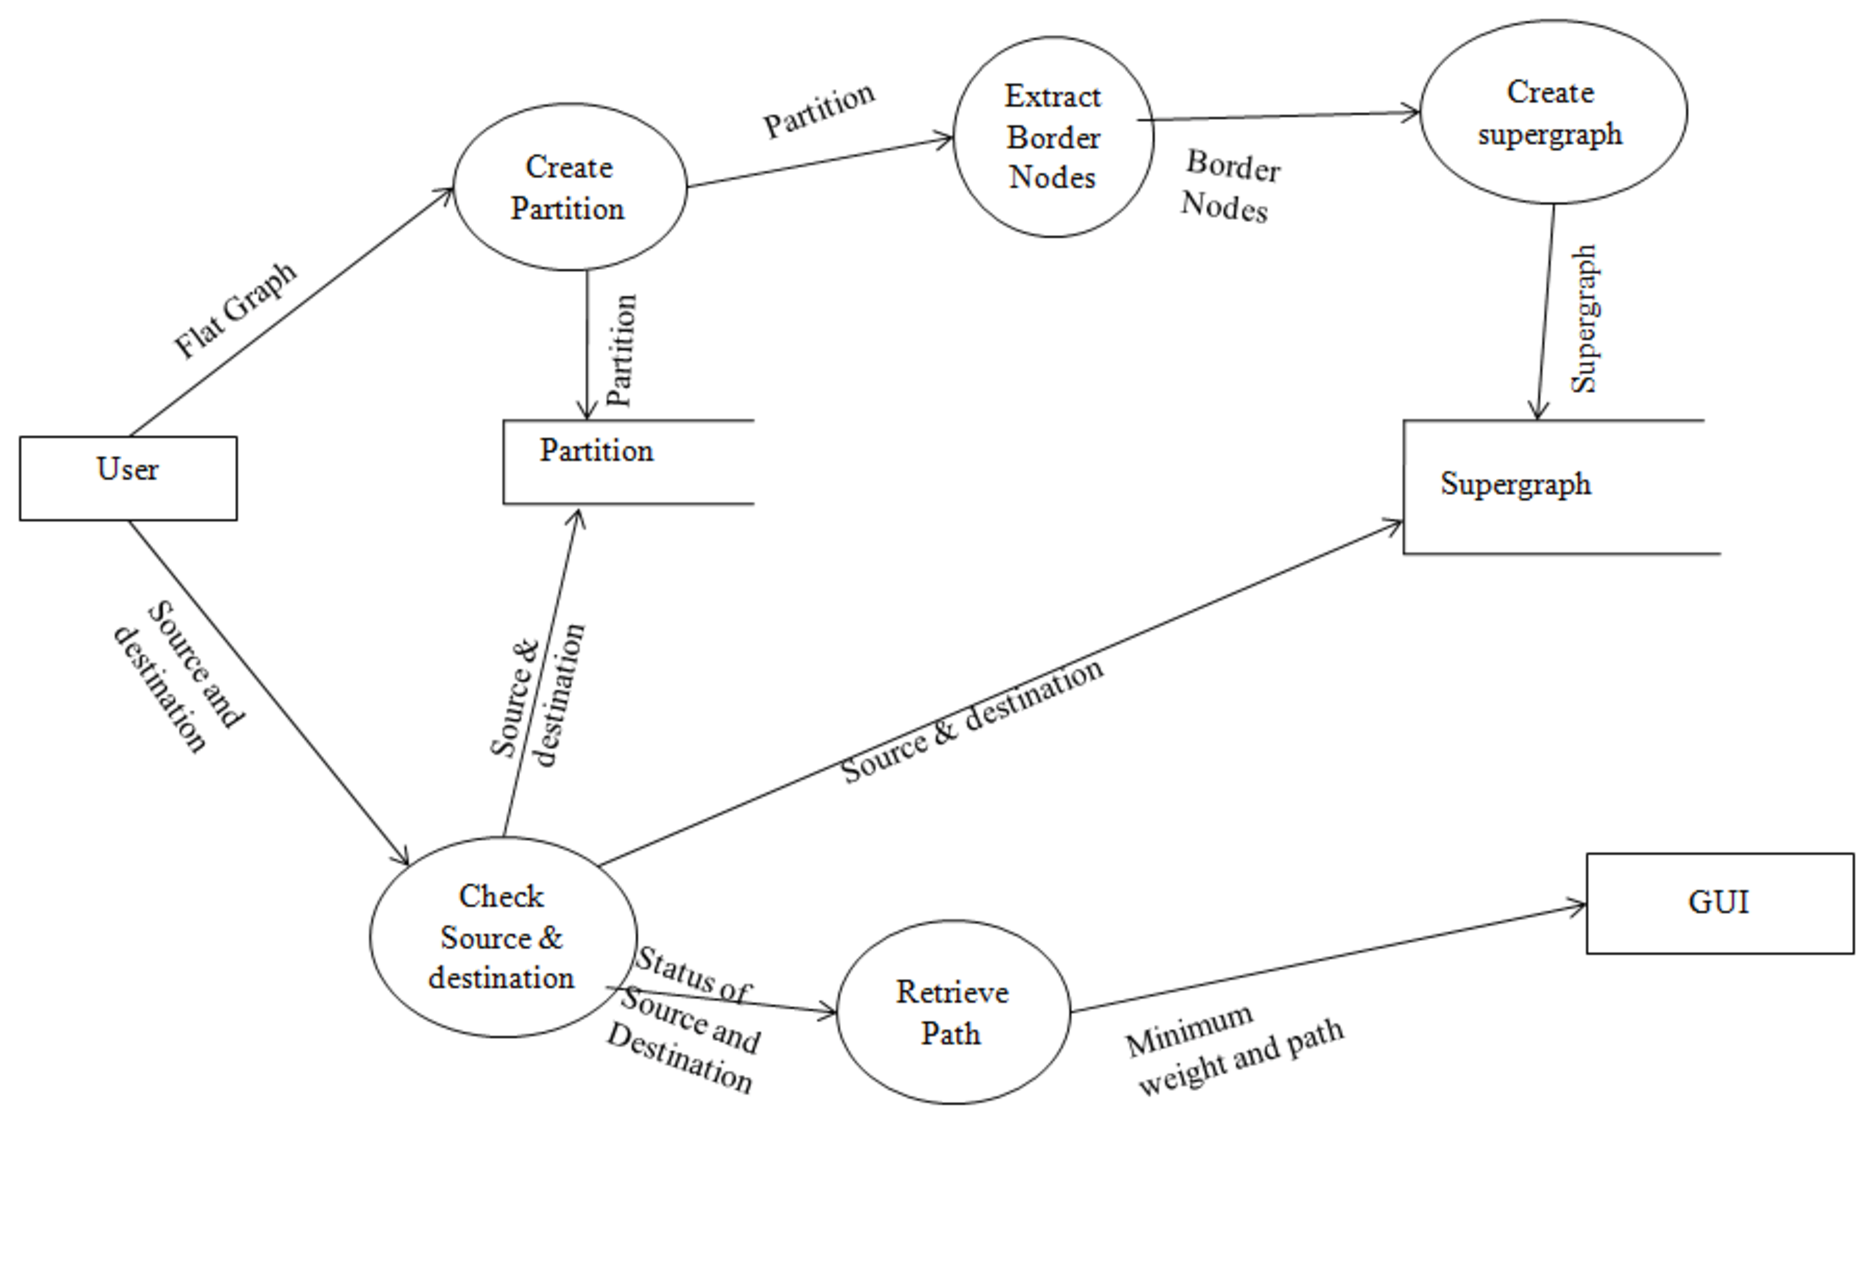
\includegraphics[width=16cm,height=10cm]{DFD.eps}
\caption{Data Flow Diagram}
\end{figure}
\newpage


\section{\normalsize ENTITY-RELATIONSHIP DIAGRAM}
\hspace{5mm} Following is the Entity Relationship Diagram which shows relationship between different entities.
\begin{figure}[H]
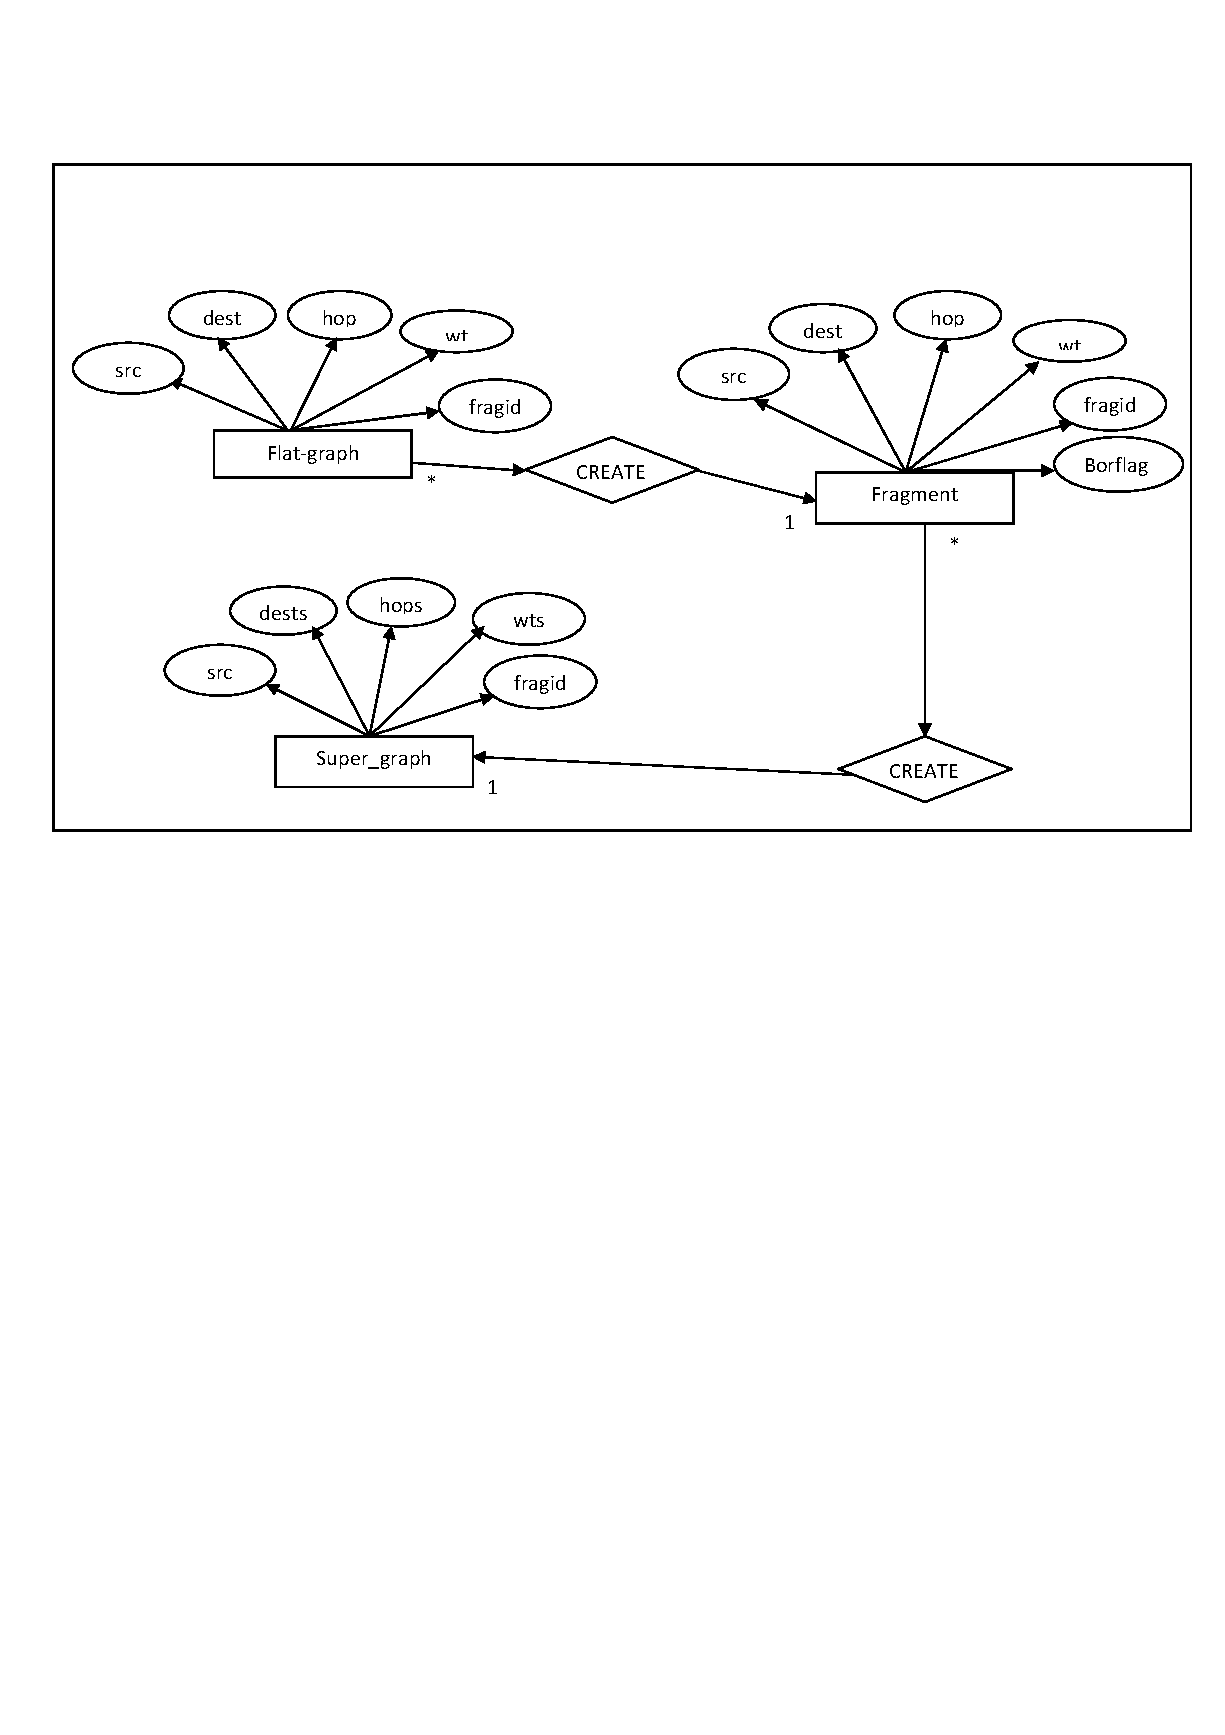
\includegraphics[width=16cm,height=15cm]{ER1.eps}
\caption{Entity-Relationship Diagram}
\end{figure}


\newpage




\section{\normalsize CLASS DIAGRAM}
\hspace*{5mm} The below diagram depicts the class diagram for image processing. System will comprise of various classes such as image, cartoon, imagesketch etc. The class diagram shows interdependency between the classes and how they communicate between them.\\
\begin{figure}[H]
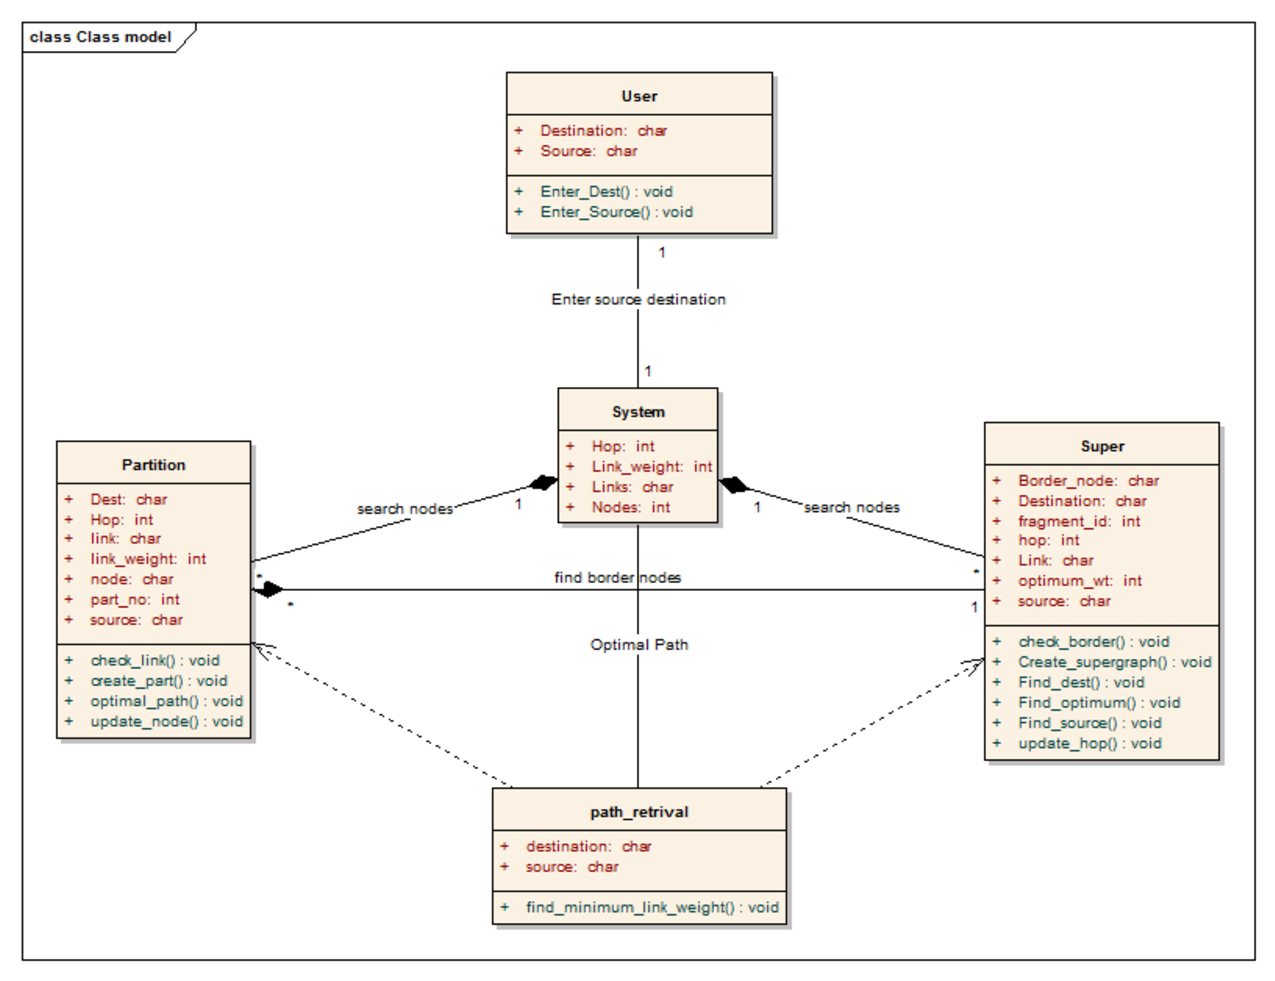
\includegraphics[width=17cm,height=17cm]{Class.eps}
\caption{Class Diagram}
\end{figure}
\newpage


\section{\normalsize SEQUENCE DIAGRAM}
\hspace{5mm} Sequence diagram represents the dynamic behaviour of the system. A Sequence diagram is a structured representation of behaviour as a series of sequential steps over time. The application’s sequence diagram shows how the elements of the application pass messages to each other during actual execution.\\
%\\ \hspace*{1cm} Following shows Sequence Diagram 
\begin{figure}[H]
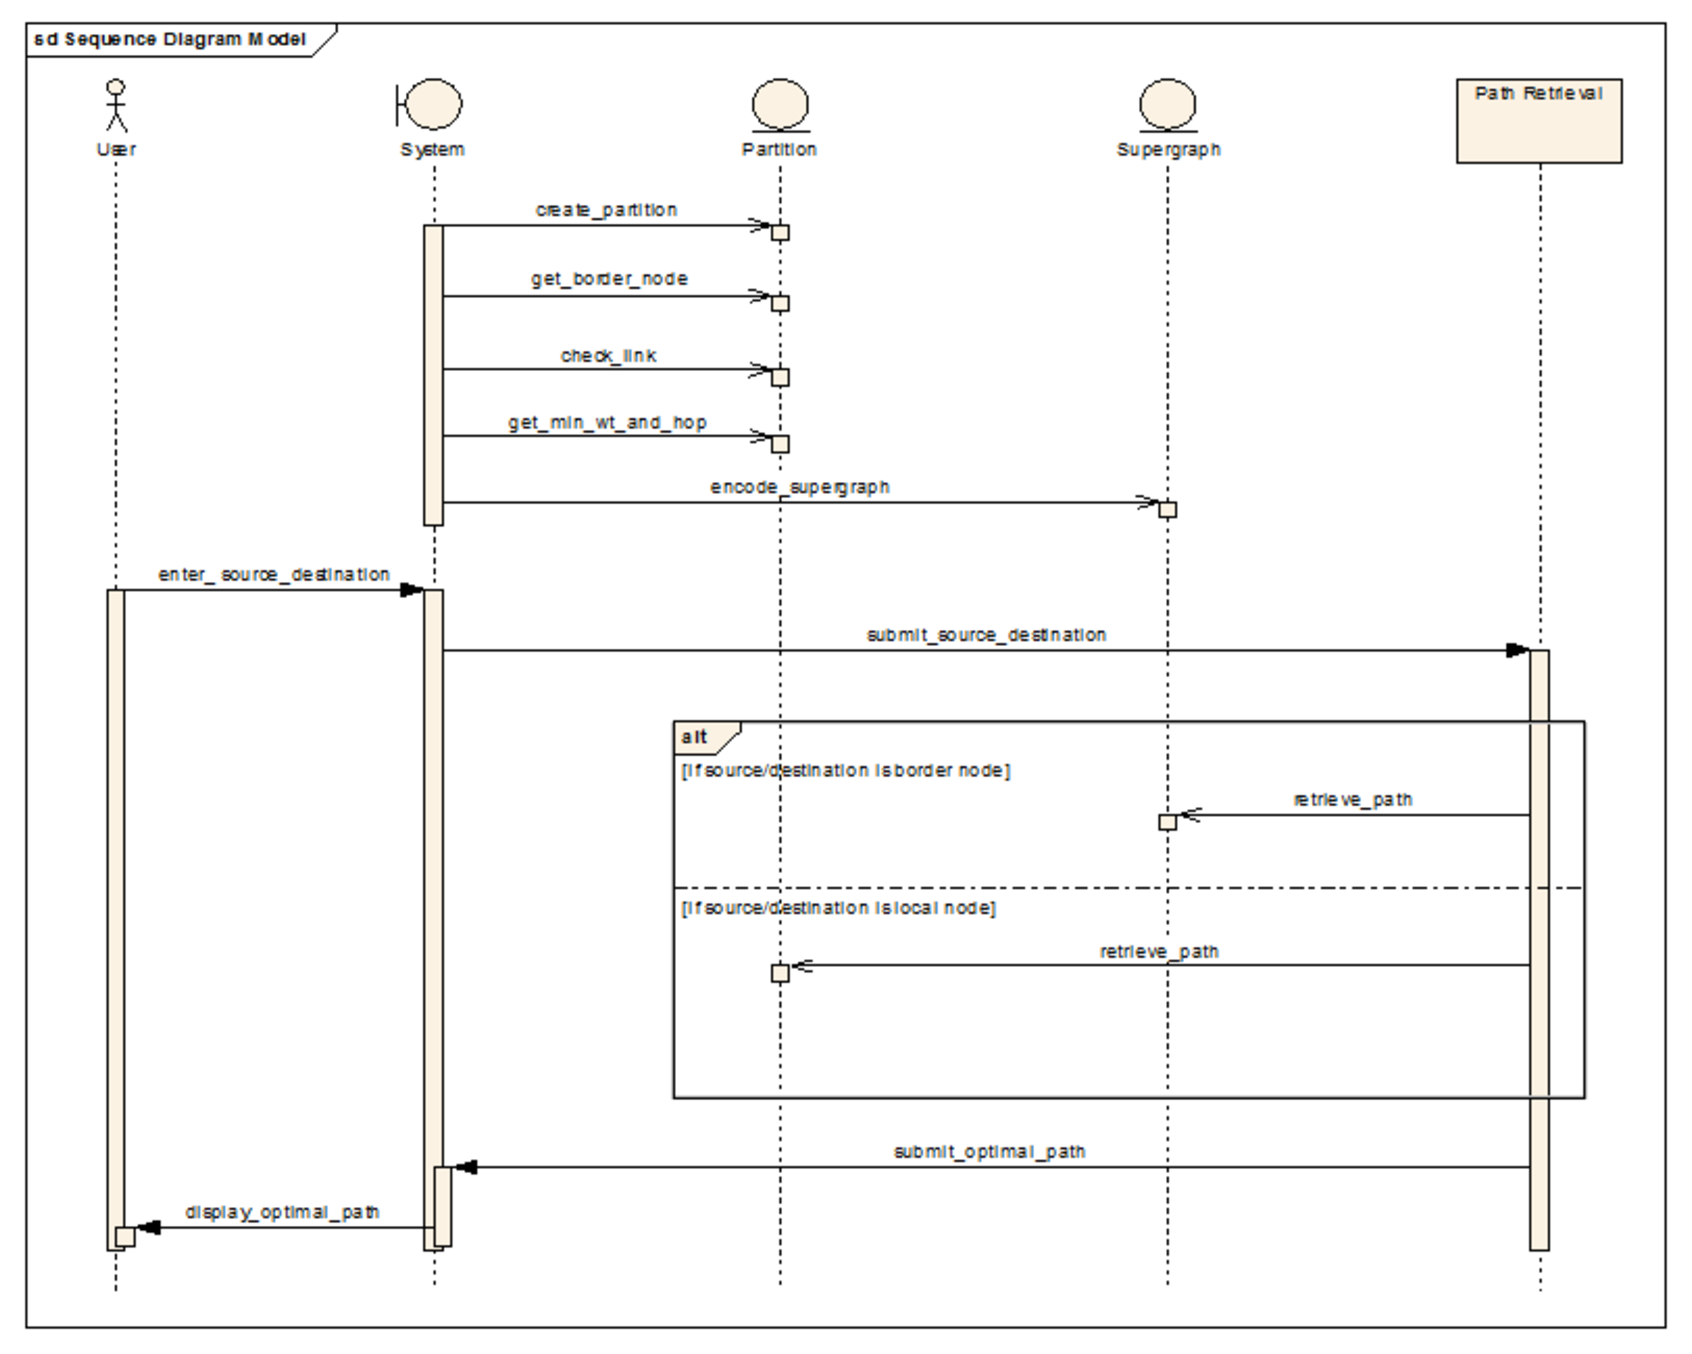
\includegraphics[width=17cm,height=17cm]{seq.eps}
\caption{Sequence Diagram}
\end{figure}
\newpage

\section{\normalsize COLLABORATION DIAGRAM}
\hspace{5mm} Following is the Collaboration diagram which shows the communication between different entities.
\begin{figure}[H]
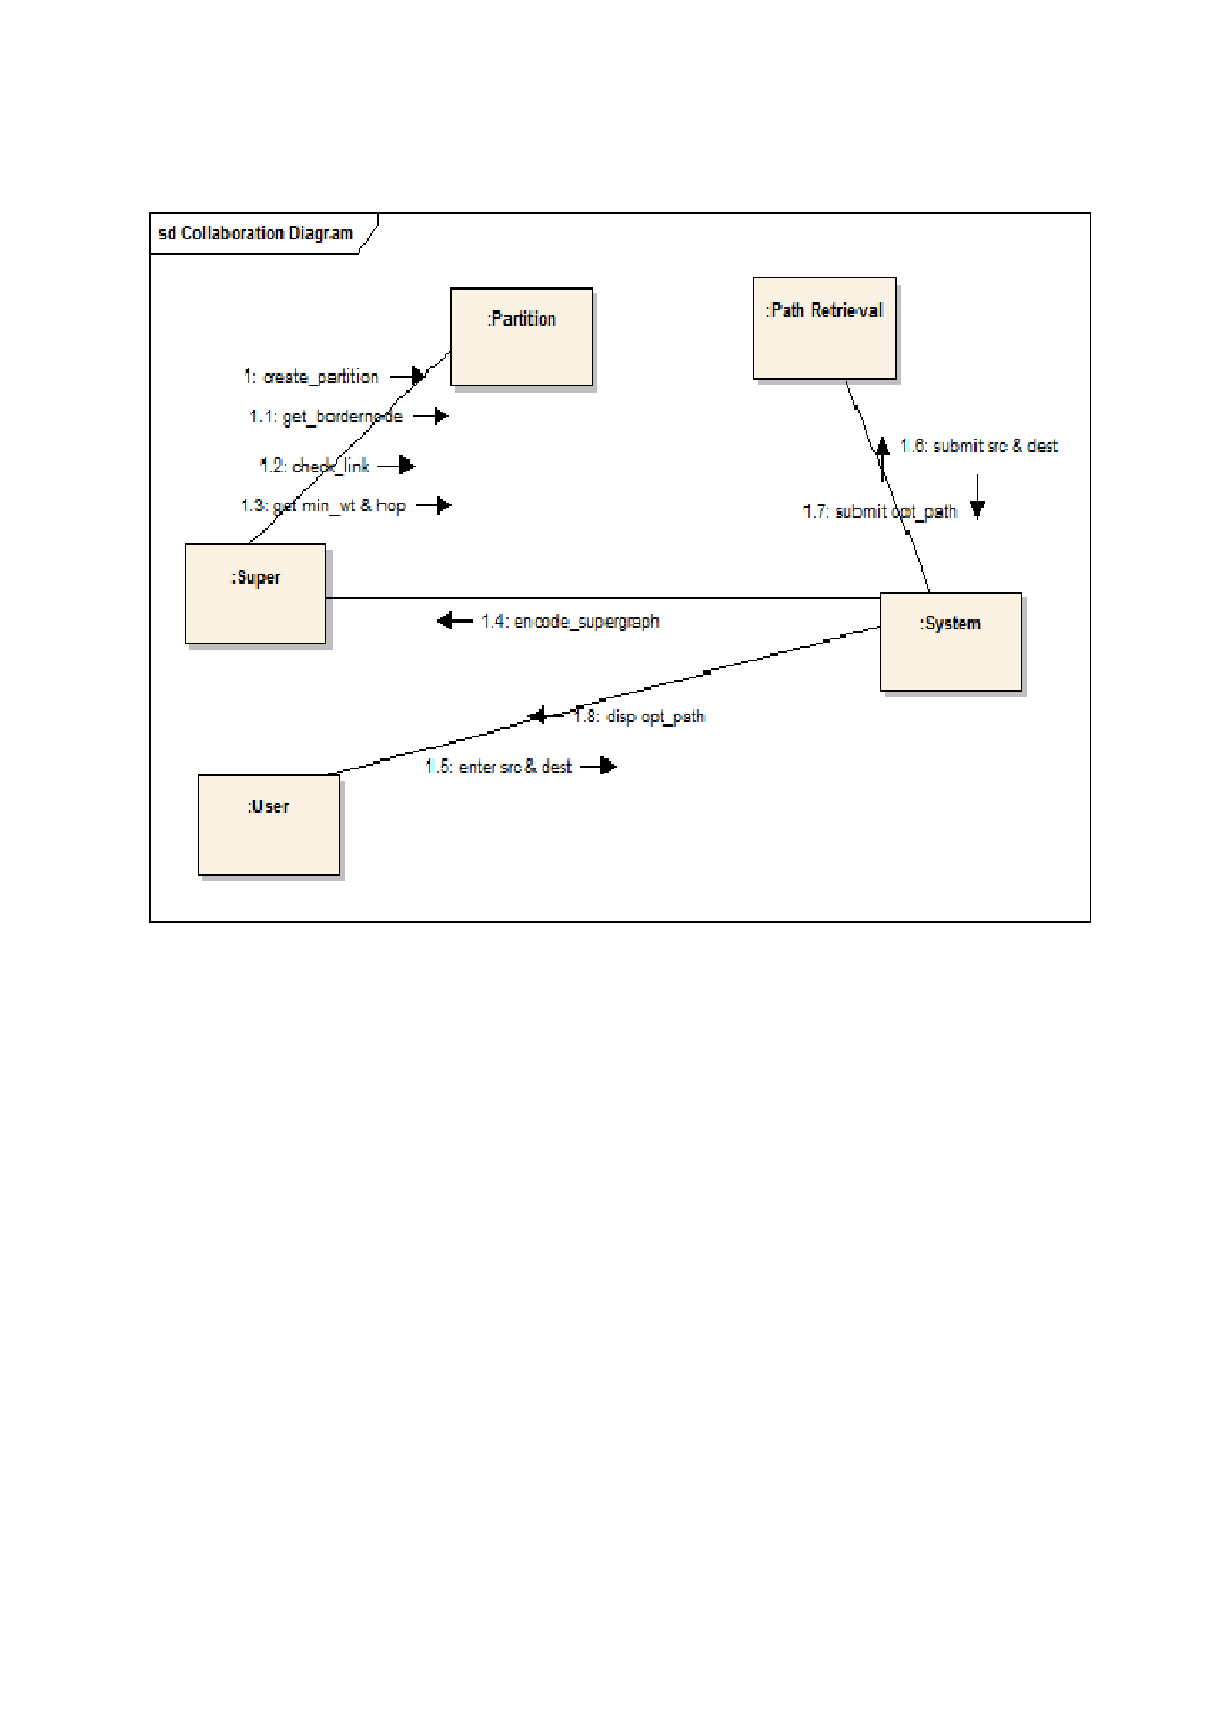
\includegraphics[width=14cm,height=20cm]{coll.eps}
\caption{Collaboration Diagram}
\end{figure}
\newpage



\section{\normalsize STATE TRANSITION}
\hspace{5mm} This diagram is a way of describing the time-dependent behavior of a system. State diagrams are used to describe the behavior of a system.  State diagrams describe all of the possible states of an object as events occur.  Each diagram usually represents objects of a single class and tracks the different states of its objects through the system.\\
%\\ \hspace*{1cm} Following is the State Transition diagram 
\begin{figure}[H]
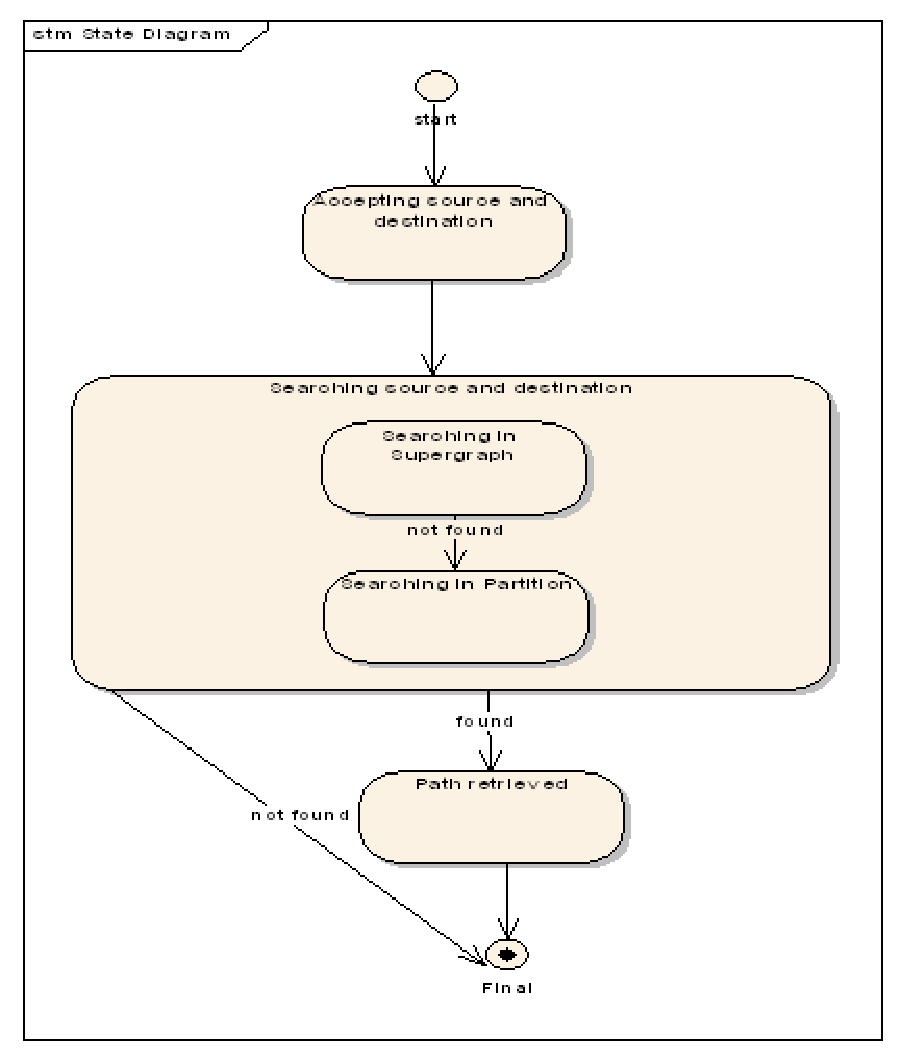
\includegraphics[width=14cm,height=17cm]{state.eps}
\caption{State Transition Diagram}
\end{figure}
\newpage


\section{\normalsize DEPLOYMENT DIAGRAM}
\hspace{5mm} A deployment diagram in the Unified Modeling Language models the physical deployment of artifacts on nodes.
\begin{figure}[H]
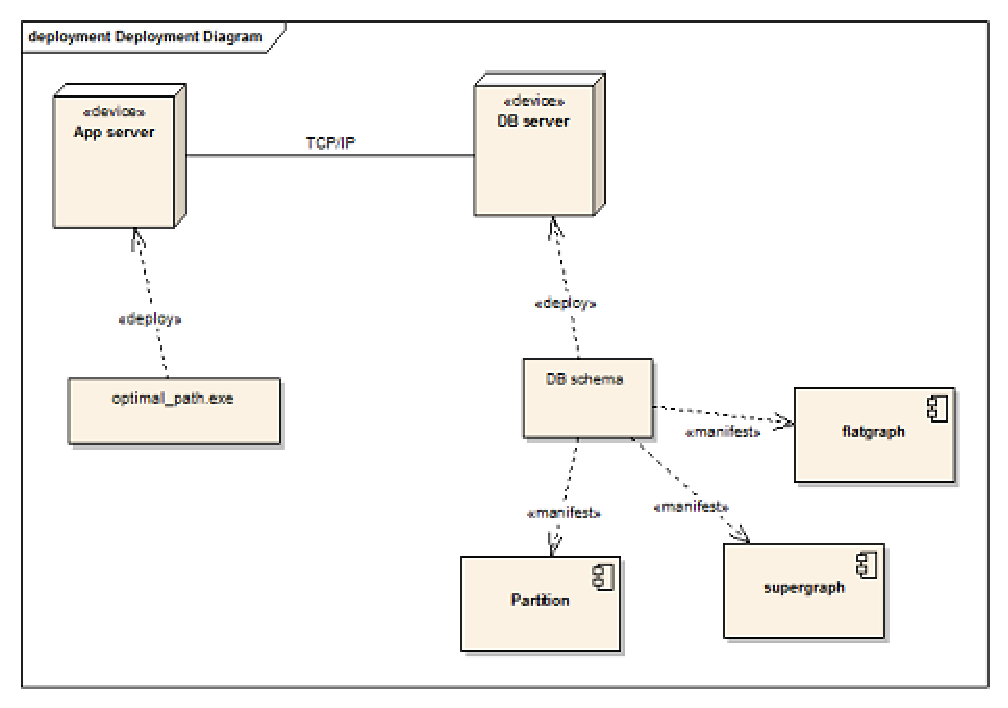
\includegraphics[width=17cm,height=17cm]{dep.eps}
\caption{Deployment Diagram}
\end{figure}
%\newpage



\end{center}
\begin{center}

\justifying
\chapter{\large PROJECT IMPLEMENTATION AND CODING}
%\begin{flushleft}
\justifying

\section{\normalsize DATABASE IMPLEMENTATION }
\hspace{1cm}The database used in this project is as given below. It gives information about the tables and their attributes.\\
\hspace*{0.7cm}\textbf{1.Source} 
\\ \hspace*{1cm}src - varchar2 - Primary Key \\

\vspace{0.2in}
\textbf{2.Map} 
\\\hspace*{1cm}src - varchar2 - Foreign Key \\
\hspace*{1cm}src name - varchar2 \\

\vspace{0.2in}
\textbf{3.Flatgraph}
\\ \hspace*{1cm}src -varchar2 - Foreign Key \\
\hspace*{1cm}dest - varchar2 \\
\hspace*{1cm}wt -float \\
\hspace*{1cm}fragid - number\\

\vspace{0.2in}
\textbf{4.frag} 
\\ \hspace*{1cm}fragid - number\\
\hspace*{1cm}src - varchar2 - Foreign Key \\
 \hspace*{1cm}hop - varchar2\\
\hspace*{1cm}wt - float  \\
\hspace*{1cm}bor - number\\

\vspace{0.2in}
\textbf{5.Supergraph} 
\\ \hspace*{1cm}src - varchar2 - Foreign Key \\
\hspace*{1cm}dests - varchar2\\
\hspace*{1cm}hops - varchar2 \\
\hspace*{1cm}wts - float \\
\hspace*{1cm}fragid - number\\

\vspace{0.2in}
\textbf{6.Login} 
\\ \hspace*{1cm}Username -varchar2- Primary Key \\
\hspace*{1cm}Password - varchar2\\
\hspace*{1cm}adminflag - number \\



\section{\normalsize GUI IMPLEMENTATION}
\begin{figure}[H]
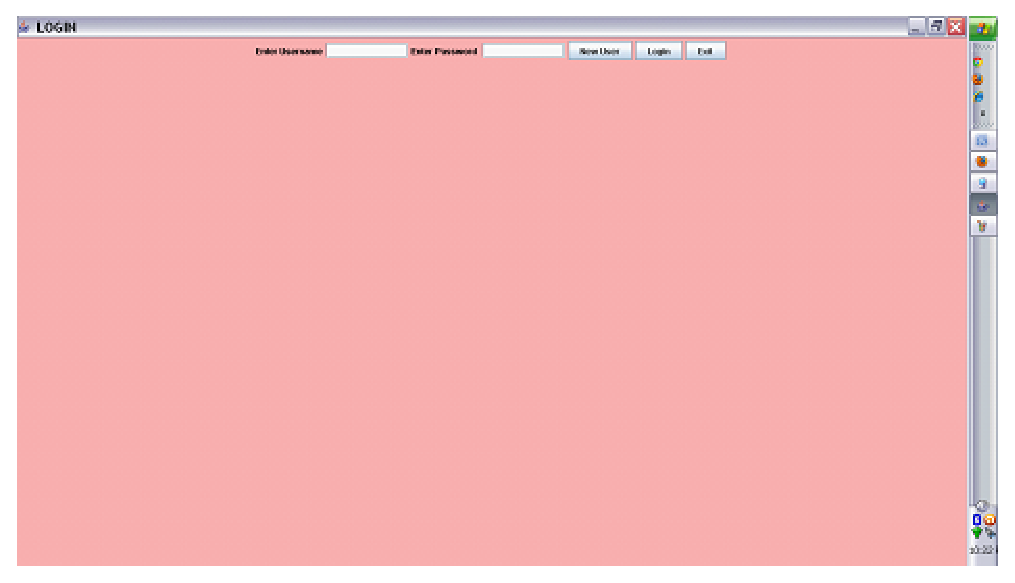
\includegraphics[width=16cm,height=13cm]{login.eps}
\caption{Login Form}
\end{figure}

\begin{figure}[H]
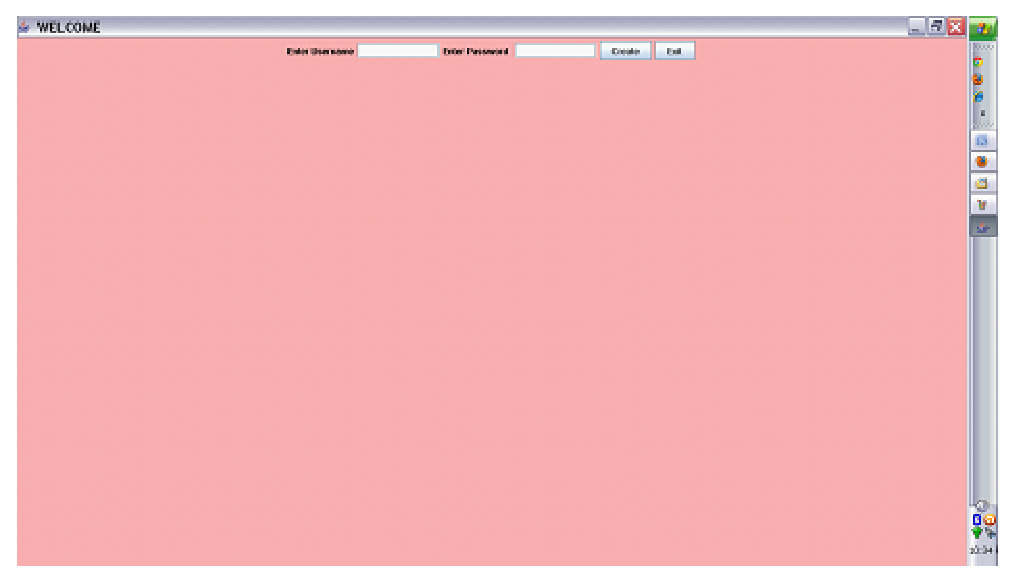
\includegraphics[width=16cm,height=13cm]{newuser.eps}
\caption{New user form}
\end{figure}

\begin{figure}[H]
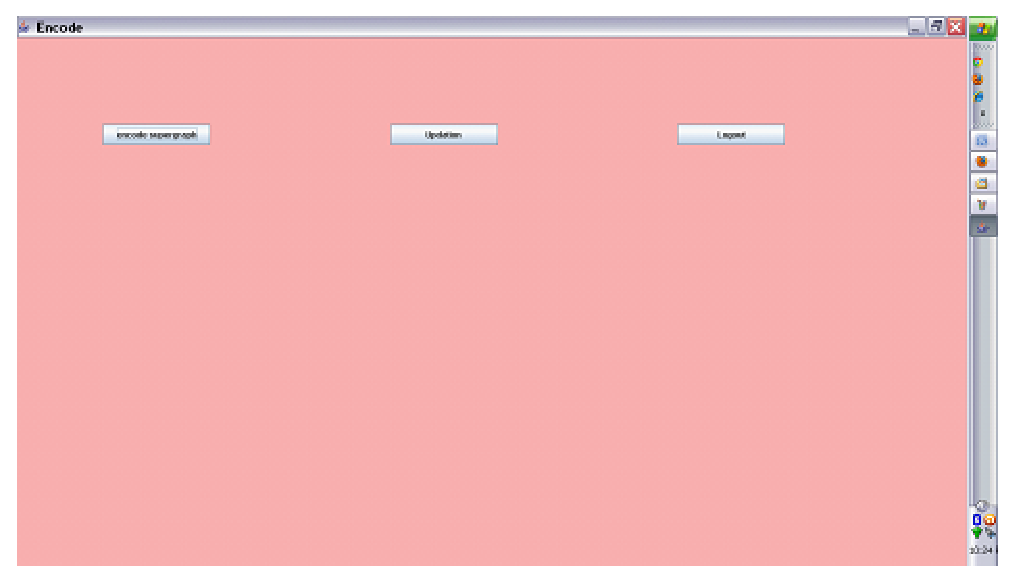
\includegraphics[width=16cm,height=13cm]{admin.eps}
\caption{Admin form}
\end{figure}

\begin{figure}[H]
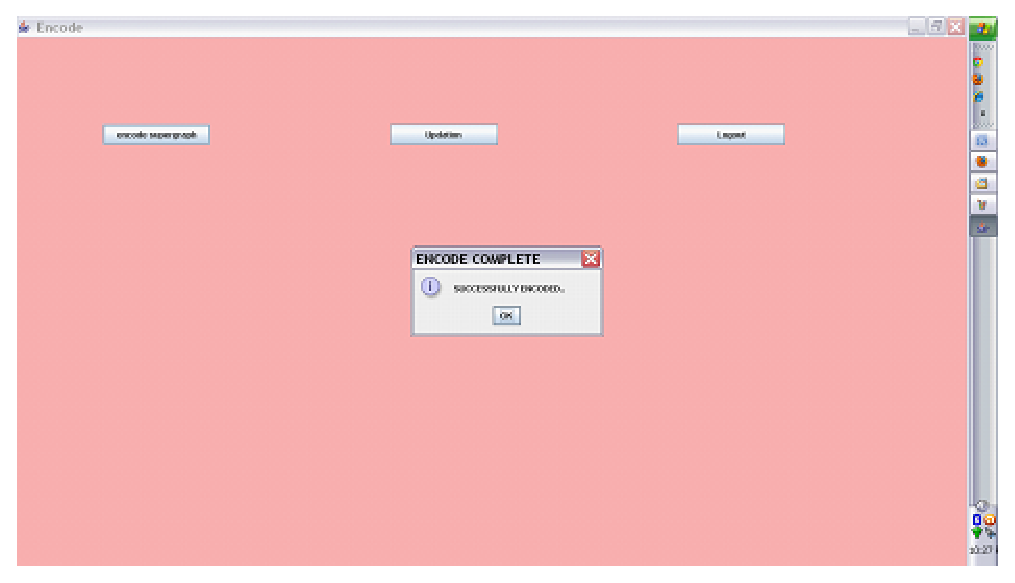
\includegraphics[width=16cm,height=13cm]{encode.eps}
\caption{Encode Form}
\end{figure}

\begin{figure}[H]
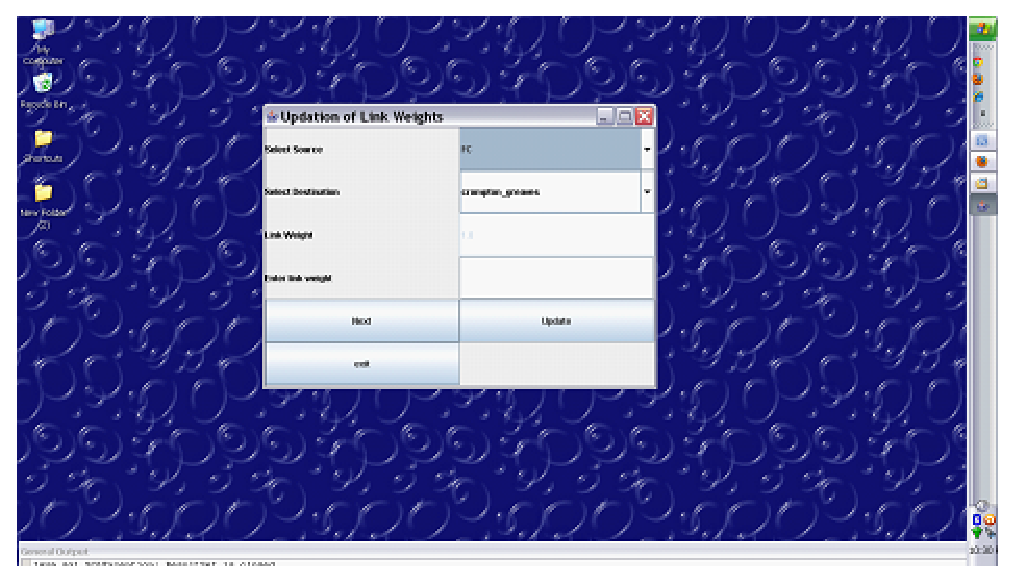
\includegraphics[width=16cm,height=13cm]{update.eps}
\caption{Update Form}
\end{figure}

\begin{figure}[H]
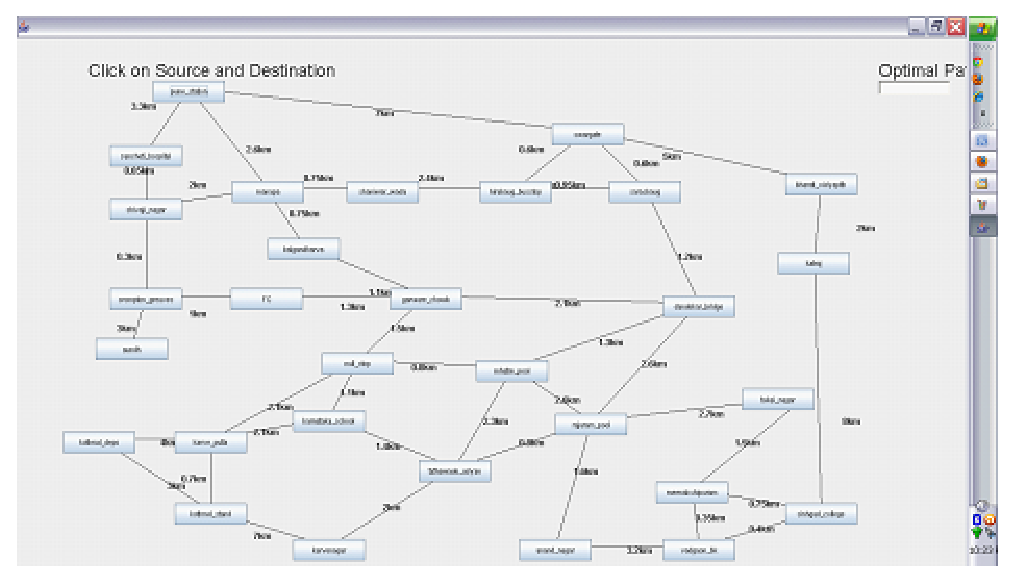
\includegraphics[width=16cm,height=13cm]{map.eps}
\caption{Map Form}
\end{figure}

\begin{figure}[H]
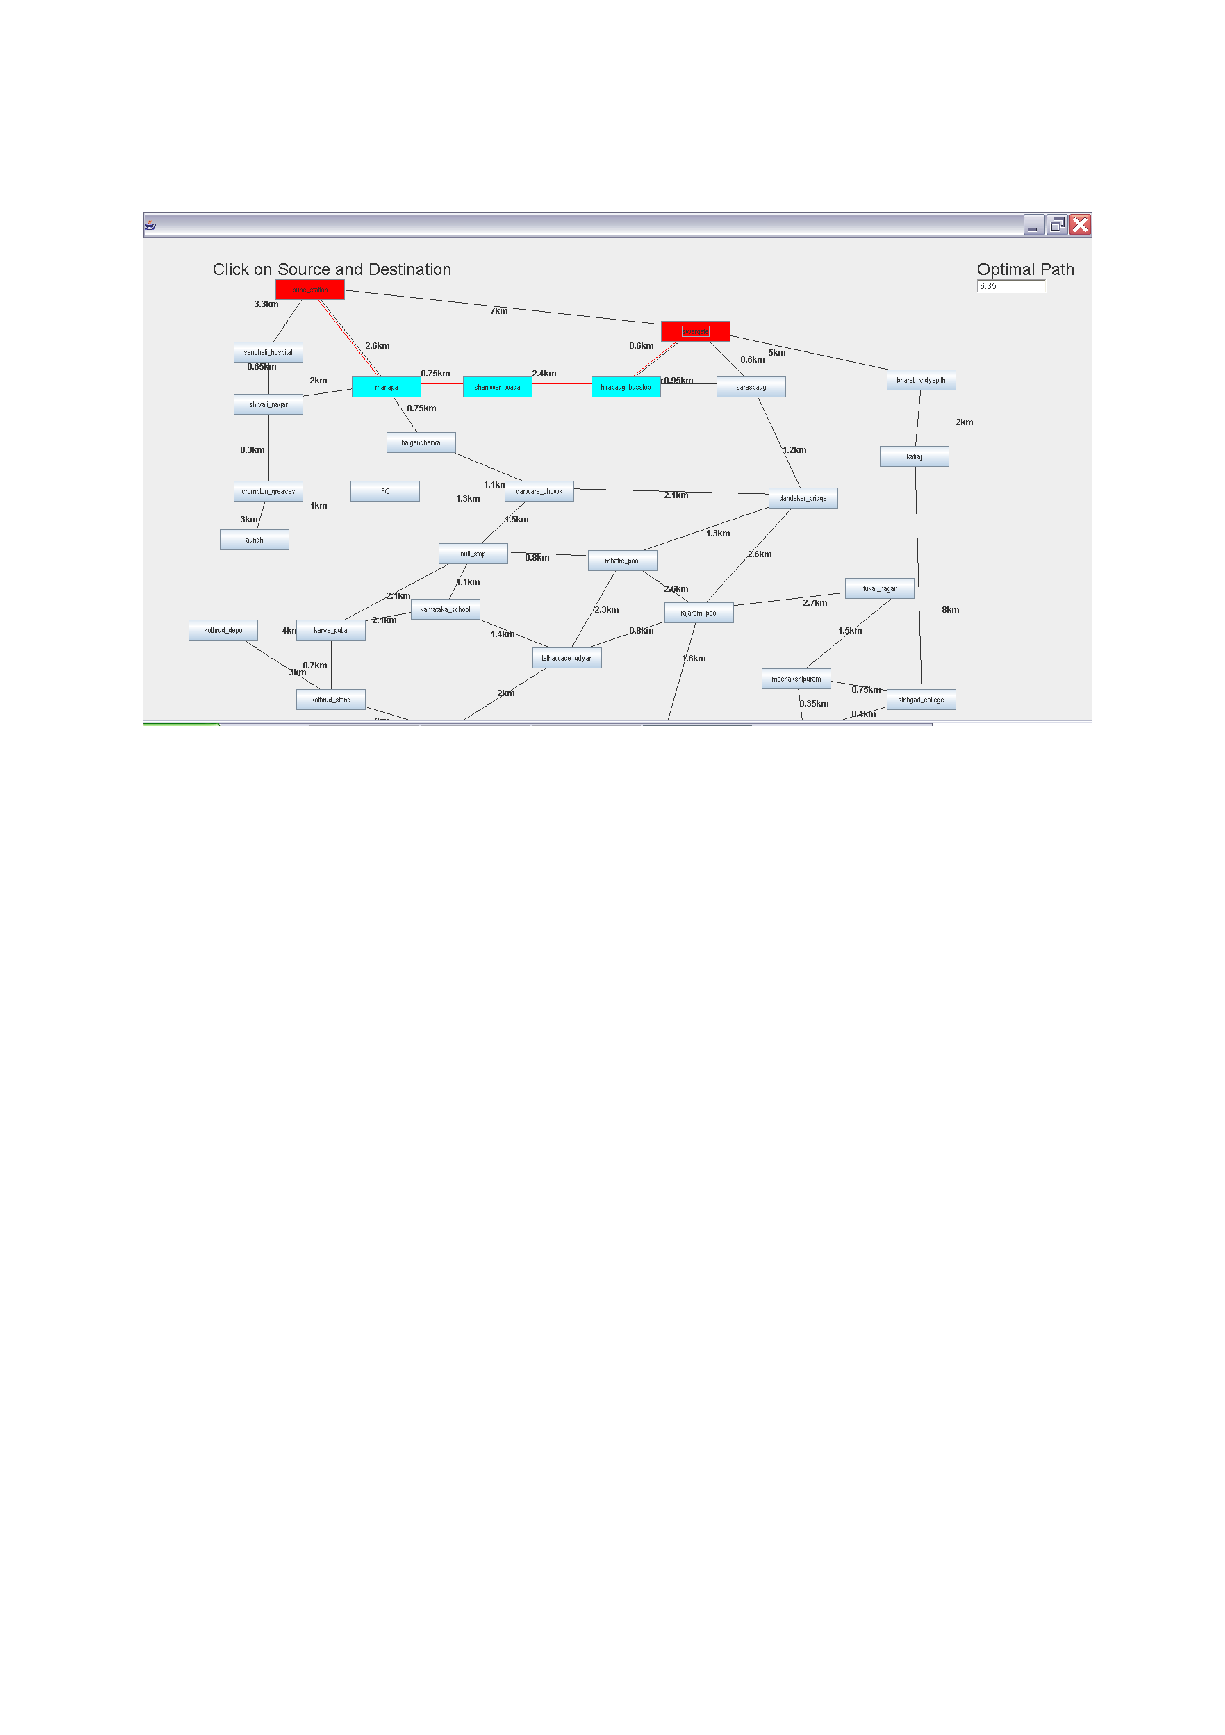
\includegraphics[width=16cm,height=36cm]{mop.eps}
\caption{Map output Form}
\end{figure}

\newpage
\section{\normalsize CODE DETAILS}
\begin{verbatim}
import java.sql.*;
import java.util.*;
import java.io.*;
import javax.swing.*;

class HEPV10
{
	private String superborder[], border[];
	int n,p,l;

	public HEPV10()
	{
		try
		{
			Class.forName("sun.jdbc.odbc.JdbcOdbcDriver");
			Connection con = DriverManager.getConnection("jdbc:odbc:HEPV","system","system");
			Statement st = con.createStatement();
			ResultSet rs = null;

			rs = st.executeQuery("select count(src) from source");	// src is primary key ...
			
			if(rs.next())
				n = rs.getInt("count(src)");
			rs.close();

			rs =st.executeQuery("select count(distinct fragid) from flat_graph");
			if(rs.next())
				p = rs.getInt("count(distinctfragid)");
			rs.close();

			rs = st.executeQuery("select count(*) from flat_graph");
			if(rs.next())
				l = rs.getInt("count(*)");
			rs.close();

			st.close();
			con.close();
		}
		catch(Exception e)
		{
			e.printStackTrace();
		}
		superborder = new String[15];
		border = new String[10];
	}

	public static void main(String[] args)
	{
		JFrame frame = new Map1("Map");
		frame.setVisible(true);
		frame.setExtendedState(frame.getExtendedState()|JFrame.MAXIMIZED_BOTH);
	}

	public void createHEPV()
	{
		Fragment frag = new Fragment();
		Supergraph superg = new Supergraph();

		borderSetting();

		for(int k = 1; k <= p; k++)		// k = fragid
		{
			encode(k);

			for(int c = 0;border[c] != null ;c++)
				border[c] = null;

			bordern(border,k);

			for(int i = 0;border[i]!=null;i++)		// border[i] = src
			{
				for(int j = 0;border[j]!=null;j++)	// border[j] = dest
				{
					if(i != j)
					{
						frag.set(border[i], border[j], k);
						superg.set(border[i], border[j],k);

						float swt, fwt;
						String fhop;

						swt = superg.getWt();
						fwt = frag.getWt();
						fhop = frag.getHop();

						if(fwt < 999.00f)
						{
							if(swt < 999.00f)
							{
								if(swt > fwt)
								{
									superg.update(fhop, fwt);
									System.out.println(" update");
								}
							}
							else
							{
								superg.insert(fhop, fwt);
								System.out.println(" insert");
							}
						}
					}
				}
			}
		}
		encode(0);	// encode supergraph
	}

	public float pathRetrieval(String src,String dest, Map1 frame)
	{
		float SPW = 999.00f;
		int flags = 0, flagd = 0;
		Fragment frag = new Fragment();
		Supergraph superg = new Supergraph();

		if(!src.equals(dest))
		{
			if(superborder[0] == null)
			{
				fillSuperborder();
			}
			for(int i = 0; superborder[i] != null; i++)
			{
				if(superborder[i].equals(src))
				{
					flags = 1; 	// src is a border node (in supergraph)
				}
				else if(superborder[i].equals(dest))
				{
					flagd = 1;	// dest is a border node (in supergraph)
				}
			}
			if(flags == 1 && flagd == 1)		// Case 1: Both src and dest nodes 
			//are border nodes (in supergraph)
			{
				try
				{
					Class.forName("sun.jdbc.odbc.JdbcOdbcDriver");
					Connection con = null;
					ResultSet rs = null;
					ResultSet rs1 = null;
					con = DriverManager.getConnection("jdbc:odbc:HEPV","system","system");
					Statement st = con.createStatement();
					rs1 = st.executeQuery("select * from super_graph 
					where src = '"+ src + "'
					and dests = '"+ dest +"'");

					if(rs1.next())
					{
						SPW = rs1.getFloat("wts");
						String hops = rs1.getString("hops");
						int fragidd = rs1.getInt("fragid");

						System.out.print(src + " -> " + hops);

						frame.highlight(src);	// colour buttons
						frame.highlight(hops);

						int fragids = 0,flag = 1;
						String hopd = null;

						rs = st.executeQuery("select fragid from frag where src  = " + src + " 
						and dest = " + hops + " and wt = (select min(wt) from frag 
						where src = " + src + " and dest = " + hops +")");

						if(rs.next())
						{
							fragids = rs.getInt("fragid");
							bordern(border, fragids);		// border[] is used for src
						}
						rs.close();

						if(fragids == fragidd && fragids != 0)	// src and dest are in same fragment
						{
							while(!hops.equals(dest))
							{
								frag.set(hops,dest,fragids);
								hops = frag.getHop();
								System.out.print(" -> " + hops);
								frame.highlight(hops);
							}
						}
						else		// traverse more than one fragment
						{
							int fragid = 0,indxs = 0;
							float min = 999.0f,wt;
							String hop = null;

							for(int i = 0;i < border.length;i++)
							{
								if(src.equals(border[i]) == false)
								{
									frag.set(hops,border[i],fragids);
									wt = frag.getWt();
									if(min > wt)
									{
										min = wt;
										indxs = i;
										hop = frag.getHop();	// hops -> hop -> border[i]
									}
								}
							}
							if(hop.equals(null) == false)
							{
								System.out.print(" -> " + hop);		// hops -> hop -> border[indxs]
								frame.highlight(hop);
								while(hop.equals(border[indxs]) == false)
								{
									frag.set(hop,border[indxs],fragids);
									hop = frag.getHop();
									System.out.print(" -> " + hop);
									frame.highlight(hop);
								}
							}
							else
							{
								System.out.print(" -> " + border[indxs]);
								frame.highlight(border[indxs]);
							}
							String[] borderd = new String[10];	// border -> borderd
							bordern(borderd, fragidd);	// borderd is used for dest
							min = 999.0f;
							int indxd = 0;
							for(int i = 0;i < borderd.length;i++)
							{
								if(border[indxs].equals(src) == false)
								{
									if(border[indxs].equals(borderd[i]))	
									// if we get same border node in fragids and fragidd
									{
										indxd = i;
										break;
									}
									else
									{
										rs = st.executeQuery("select fragid from super_graph
										where src = " + border[indxs] + " and dests = " + borderd[i]);
										if(rs.next())
											fragid = rs.getInt("fragid");
										frag.set(border[indxs],borderd[i],fragid);
										wt = frag.getWt();
										if(min > wt)
										{
											min = wt;
											hop = frag.getHop();
											indxd = i;
										}
										rs.close();
									}
								}
							}
							if(border[indxs].equals(borderd[indxd]) == false)	
							// 2 different border nodes in different fragment
							{
								while(!hop.equals(borderd[indxd]))
								{
									frag.set(hop,borderd[indxd],fragid);
									hop = frag.getHop();
									System.out.print(" -> " + hop);
									frame.highlight(hop);
								}
							}
							hopd = borderd[indxd];
							while(!hopd.equals(dest))
							{
								frag.set(hopd,dest,fragidd);
								hopd = frag.getHop();
								System.out.print(" -> " + hopd);
								frame.highlight(hopd);
							}
						}
					}
					else
						SPW = 999.0f;
					st.close();
					con.close();
				}
				catch(Exception e)
				{
					System.out.println(e);
				}
			}
			else if(flags == 1 && flagd == 0)	// Case 2: The src is a border node
			//, but the dest is a local node (in fragment)
			{
				try
				{
					Class.forName("sun.jdbc.odbc.JdbcOdbcDriver");
					Connection con = null;
					ResultSet rs = null;
					ResultSet rs1 = null;
					ResultSet rs2 = null;
					con = DriverManager.getConnection("jdbc:odbc:HEPV","system","system");
					Statement st = con.createStatement();
					rs = st.executeQuery("select * from super_graph 
					where src = '" + src + "'");
					if(rs.next())
					{
						int fragids = 0,fragidd = 0;
						String hop = null;

						for(int j = 1;j <= p;j++)
						{
							rs1 = st.executeQuery("select * from frag 
							where fragid = " + j + " and dest = " + dest + " and bor = 0");
							if(rs1.next())
							{
								fragidd = j;
								bordern(border, fragidd);

								float swt = 0.00f,fwt = 0.00f;

								for(int k = 0; border[k]!= null; k++)
								{
									superg.set(src,border[k],0);
									frag.set(border[k],dest,fragidd);

									swt = superg.getWt();
									fwt = frag.getWt();

									if((swt + fwt) < SPW)
									{
										hop = border[k];
										rs2 = st.executeQuery("select fragid from super_graph 
										where src  = '" + src + "' and dests = '" + border[k] + "'");
										if(rs2.next())
										{
											fragids = rs2.getInt("fragid");
										}
										rs2.close();
										SPW = swt + fwt;
									}
								}
								System.out.print(src);
								frame.highlight(src);
								while(!src.equals(hop))
								{
									frag.set(src,hop,fragids);
									src = frag.getHop();
									System.out.print(" -> " + src);
									frame.highlight(src);
								}
								while(!hop.equals(dest))
								{
									frag.set(hop,dest,fragidd);
									hop = frag.getHop();
									System.out.print(" -> " + hop);
									frame.highlight(hop);
								}
								rs1.close();
								break;
							}
						}
					}
					rs.close();
					st.close();
					con.close();
				} //try
				catch(Exception e)
				{
					System.out.println(e);
				}
			}
			
			else		// Case 3: Both the src and dest nodes are local nodes (in fragment)
			{
				try
				{
					int flag = 0;
					String hops = null,hopd = null;

					Class.forName("sun.jdbc.odbc.JdbcOdbcDriver");
					Connection con = null;
					ResultSet rs = null;
					ResultSet rs1 = null;
					con = DriverManager.getConnection("jdbc:odbc:HEPV","system","system");
					Statement st = con.createStatement();
					int fragids = 0,fragidd = 0;

					for(int i = 1; i <= p; i++)
					{
		rs = st.executeQuery("select * from frag 
		where fragid = " + i + " and src = '" + src + "'");
						if(rs.next())
						{
							bordern(border, i);		// border[] is used for src
							fragids = i;
							rs.close();
							break;
						}
						rs.close();
					}
					String[] borderd = new String[10];
					for(int j = 1; j <= p; j++)
					{
		rs = st.executeQuery("select * from frag 
		where fragid = " + j + " and dest = '" + dest + "'");
						if(rs.next())
						{
							bordern(borderd, j);	// borderd is used for dest
							fragidd = j;
							rs.close();
							break;
						}
						rs.close();
					}
					if(fragids!=0 && fragidd!=0)
					{
						float swt,fwts,fwtd;

						for(int i = 0; border[i]!= null; i++)
						{
							for(int j = 0; borderd[j]!=null; j++)
							{
								frag.set(src,border[i],fragids);
								fwts = frag.getWt();
								superg.set(border[i],borderd[j],0);
								swt = superg.getWt();
								frag.set(borderd[j], dest,fragidd);
								fwtd = frag.getWt();
								if((swt + fwts + fwtd) < SPW)
								{
									hops = border[i];
									hopd = borderd[j];
									SPW = swt + fwts + fwtd;
									flag = 1;
								}
							}
						}
					}
					if(fragids == fragidd && fragids != 0)
					{
						float fwt;

						frag.set(src,dest,fragids);
						fwt = frag.getWt();
						if(fwt < SPW)
						{
							hops = frag.getHop();
							SPW = fwt;
							flag = 2;
						}
					}
					if(flag == 1)
					{
						int fragid = 0;

						System.out.print(src);
						frame.highlight(src);

						while(!src.equals(hops))
						{
							frag.set(src,hops,fragids);
							src = frag.getHop();
							System.out.print(" -> " + src);
							frame.highlight(src);
						}

						rs = st.executeQuery("select fragid from super_graph 
						where src = '" + hops + "' and dests = '" + hopd + "'");
						if(rs.next())
						{
							fragid = rs.getInt("fragid");
						}

						while(!hops.equals(hopd))
						{
							frag.set(hops,hopd,fragid);
							hops = frag.getHop();
							System.out.print(" -> " + hops);
							frame.highlight(hops);
						}

						while(!hopd.equals(dest))
						{
							frag.set(hopd,dest,fragidd);
							hopd = frag.getHop();
							System.out.print(" -> " + hopd);
							frame.highlight(hopd);
						}
					}
					else if(flag == 2)
					{
						System.out.print(src + " -> " + hops);
						frame.highlight(src);
						frame.highlight(hops);

						while(!hops.equals(dest))
						{
							frag.set(hops,dest,fragids);
							hops = frag.getHop();
							System.out.print(" -> " + hops);
							frame.highlight(hops);
						}
					}

					rs.close();
					st.close();
					con.close();
				} //try
				catch(Exception e)
				{
					System.out.println(e);
				}
			}
		}
		else
System.out.println("Source and Destination are same. Thus, shortest distance = 0.0");

		return SPW;
	}
	private int flatUpdate(String src, String dest,float linkwt)
	{
		int fragid = 0;

		try
		{
			Class.forName("sun.jdbc.odbc.JdbcOdbcDriver");
			Connection con = null;
			ResultSet rs = null;
			con = DriverManager.getConnection("jdbc:odbc:HEPV","system","system");
			Statement st = con.createStatement();
st.executeUpdate("Update flat_graph set wt = " + linkwt + " 
where src = '" + src + "' and dest = '" + dest + "'");
rs = st.executeQuery("select fragid from flat_graph 
where src = '" + src + "' and dest = '" + dest + "'");
			if(rs.next())
			{
				fragid = rs.getInt("fragid");
			}
			rs.close();

			st.close();
			con.close();
		}
		catch(Exception e)
		{
			System.out.println(e);
		}
		return fragid;
	}

	public void HEPVUpdate()
	{
		int fragid[] = new int[p];
		String ch, borderc[] = new String[10], bor[] = new String[10];

		for(int i = 0; i < p; i++)
			fragid[i] = 0;

		do
		{
			Scanner sc = new Scanner(System.in);

			System.out.println("Enter src: \t");
			String src = sc.nextLine();

			System.out.println("Enter dest: \t");
			String dest = sc.nextLine();

			System.out.println("Enter new linkwt:\t");
			float linkwt = Float.parseFloat(sc.nextLine());

			int id = flatUpdate(src,dest,linkwt);
			fragid[--id] = 1;

			System.out.println("Do you want change any links?");
			ch = sc.nextLine();

		}while(ch == "y");


		for(int i = 0; i < p; i++)
		{
			if(fragid[i] == 1)
				encode(i+1);
		}


		for(int i = 0; border[i]!= null; i++)
		{
			border[i] = null;
			borderc[i] = null;
		}

		for(int i = 0; i < p; i++)
		{
			if(fragid[i] == 1)
			{
				bordern(border,i+1);

				for(int j = 0; border[j] != null; j++)
				{
					for(int k = 0; border[k] != null; k++)
					{
						if(j != k)
						{
							Supergraph superg = new Supergraph();
							superg.set(border[j], border[k], i+1);
							superg.update(null,999.00f);
						}
					}
				}
			}
		}

		for(int k = 1; k <= p; k++)
		{
			for(int i = 0; border[i]!=null; i++)
			{
				border[i] = null;
			}
			bordern(border,k);

			for(int l = 0; l < p; l++)
			{
				if(fragid[l] == 1)
				{
					for(int i = 0; borderc[i] != null; i++)
					{
						borderc[i] = null;
					}
					bordern(borderc,l+1);

					int c = 0;

					for(int u =0; border[u] != null;u++) 
					// create bor[] for Ni, Nj that belong to both //border[] and borderc[]
					{
						for(int v = 0; borderc[v] != null;v++)
						{
							if(border[u] == borderc[v])
							{
								int i;
								for(i = 0; bor[i] != null; i++) // no duplicate entries
								{
									if(bor[i] == border[u])
										break;
								}
								if(bor[i] == null)
									bor[c++] = border[u];
							}
						}
					}

					for(int i = 0; bor[i] != null; i++)
					{
						for(int j = 0; bor[j] != null; j++)
						{
							if(bor[i] != bor[j])
							{
								Supergraph superg = new Supergraph();
								Fragment frag = new Fragment();

								superg.set(bor[i], bor[j], l+1);
								frag.set(bor[i], bor[j], l+1);

								float fwt = frag.getWt();
								float swt = superg.getWt();

								if(fwt < 999.00f && swt > fwt)
								{
									superg.update(frag.getHop(),fwt);
								}
							}
						} // for j
					} // for i
				}
			} // for l
		} // for k

		encode(0);	// encode supergraph
	}
}
\end{verbatim}







\begin{center}

\justifying
\chapter{\large PROJECT TESTING}

\justifying
\section{\normalsize MANUAL TESTING}
\tabletail{% 
	\hline}

		\begin{supertabular}{| p{1.73cm} |p{1.73cm}| p{1.73cm}| p{1.73cm} | p{1.73cm} | p{1.73cm} | p{1.73cm} | p{1.73cm} |}
		 \hline
  \textbf{Test Case ID}  &	\textbf{Test Case Name} &	\textbf{Test Case Description} &	\textbf{Steps} & \textbf{Expected Result} & \textbf{Actual Result} &\textbf{Test Status(P/F)} & \textbf{Test Priority}\\ \hline
			Login01 & Login & To verify username and password & Enter invalid username and valid password & An error message "Enter valid username & An error massage Displayed & P & high \\ \hline
			Login02 & Login1 & To verify username and password & Enter valid username and valid password & Next Form shoule display & Next form displayed & P & high \\ \hline
			Encode01 & Encode & To check whether fragment is encoded & Click on Encode button &  A message "successfully Encoded" display Fragment gets encoded & Successfully Encoded & P & high \\ \hline
			Encode02 & Encode1 & To check whether supergraph is created & Click on Encode button &  A message "successfully Encoded" display. supergraph is created & Successfully Encoded. Supergraph created & P & high \\ \hline
			Update01 & Update & To check whether database upadated & click on update button & A message "Successfully Updated" should display. Database updated & A message not displayed. Database not updated. & F & medium \\ \hline
			
			PathDisplay01 & PathDisplay & To verify proper path display & Select source and destination & The path between source and destination get hidglighted & Path is highlighted & P & high \\ \hline
			Distance01 & Distance & To verify shortest distance display & select source and destination & The shortest distance displayed & The shortest distance not displayed & F & high \\ \hline
	
		\end{supertabular}
\end{center}
\chapter{\large CONCLUSION}
%\begin{flushleft}
\justifying

\hspace*{1cm}Implemented hierarchical graph model supports efficient optimal path retrieval. By extending the encoded path view to the hierarchical graph model, we achieve an excellent compromise between the complete computations of paths on-demand versus precomputing all paths. Path retrieval is still significantly faster than A*. In addition, the memory requirement of HEPV is also much less compared to FEPV.\\

\textbf{The contributions of our project can be summarized as follows:}\\
 \hspace*{1cm}1.	Implemented hierarchical graph model (HEPV) exploits path materialization strategies.\\
 \hspace*{1cm}2.	These algorithms are used to create and maintain HEPV.\\
 \hspace*{1cm}3.	Implemented a shortest path retrieval algorithm which can be shown to be optimal.\\


%\end{flushleft}
%\begin{flushleft}

\chapter{\large REFERENCES}

%\section{\normalsize IEEE-I}
%\justifying
%\lipsum[1]

%\textbf{Title :}	Hierarchical Optimization of Optimal Path Finding for Transportation
%Applications \\
%\textbf{Authors :}\\
%\hspace*{2cm}Ning Jing................University of Michigan \\
%\hspace*{2cm}Yun-Wu Huang.........	University of 	Michigan\\
%\hspace*{2cm}Elke Rundensteiner.....University of Michigan\\

%\section{\normalsize IEEE-II}


%\textbf{Title :}	Direct transitive closure algorithms: design and performance evaluation\\
%\textbf{Authors :}\\
%\hspace*{2cm}Rakesh Agarwal.....AT and T Bell Labs, Murray Hill, NJ\\
%\hspace*{2cm}Shaul Dar..............AT and T Bell Labs, Murray Hill, NJ\\
%\hspace*{2cm}H. V. Jagdish.........AT and T Bell Labs, Murray Hill, NJ\\

\hspace{0cm}[1] Ning Jing, Yun-Wu Huang, Elke Rundensteiner "Hierarchical Optimization of Optimal Path Finding for Transportation Applications,"\\
\hspace{1cm}[2] R. Agrawal, S. Dar and H. V. Jagadish, �Direct Transitive Closure Algorithms: Design and Performance Evaluation,� ACM TODS, Vol. 15, No. 3, Sep. 1990, pp. 427 � 458.\\
\hspace{1cm}[3] R. Agrawal and H. V. Jagadish, �Hybrid Transitive Closure Algorithms,� Proc. of the 16th VLDB Conf., 1990, pp. 326 � 334. \\
\hspace{1cm}[4] T. Cormen, C. Leiserson, and R. L. Rivest, �Introduction to Algorithms,� The MIT Press, 1993. \\
\hspace{1cm}[5] M. A.W. Hustma, F. Cacace, and S. Ceri, �Parallel Hierarchical Evaluation of Transitive Closure Queries,� Proc. of the 1st Int. Conf. on Parallel and Distributed Information Systems, 1990, pp. 130 � 137.\\

%\end{flushleft}
\end{center}

\end{document}
